\subsection{Graphical user interface}
GUI was written in React framework.

\subsubsection{Connection with backend}
Connection with RestAPI was realized by HTTP requests like \textit{POST}, \textit{PUT}, \textit{GET}, \textit{DELETE}. Example of \textit{POST} and \textit{PUT} requests are in listing \ref{lst:GUIBackendConnector}.

\begin{lstlisting}[breaklines=true, numbers=left, stepnumber=1, label={lst:GUIBackendConnector}, caption={Connection with backend through RestAPI}]
token: auth.authState.token
}
setSaveLoadingBookFullDetailsForm(true);
const { data } = credentials.id ? (
  await fetchContext.authAxios.put(
    `/book/` + credentials.id + '?' + qs.stringify(queryValues),
    saveBookItem
  )
) : (
    await fetchContext.authAxios.post(
      `/book?` + qs.stringify(queryValues),
      saveBookItem
    )
  );
\end{lstlisting}

\subsubsection{Sidebar}
Main navigation element of web app is sidebar. It changes according to logged in user. Each of user type has different set of visible buttons on sidebar. Listing \ref{lst:GUISidebarElements} contains possible endpoints with label and allowed role for each button. Button will be visible only when user type will be included in allowedRoles array.

\begin{lstlisting}[breaklines=true, numbers=left, stepnumber=1, label={lst:GUISidebarElements}, caption={Sidebar buttons with allowed user types}]
const navItems = [
  {
    label: 'components.sidebar_component.link_label.find_books',
    path: '/find-books',
    icon: faBook,
    allowedRoles: [reader, librarian]
  },
  {
    label: 'components.sidebar_component.link_label.orders',
    path: '/manage-orders',
    icon: faBookOpen,
    allowedRoles: [reader]
  },
  {
    label: 'components.sidebar_component.link_label.manage_books',
    path: '/manage-books',
    icon: faEdit,
    allowedRoles: [librarian]
  },
  {
    label: 'components.sidebar_component.link_label.manage_orders',
    path: '/manage-orders',
    icon: faTasks,
    allowedRoles: [librarian]
  },
  {
    label: 'components.sidebar_component.link_label.all_users',
    path: '/users',
    icon: faUsersCog,
    allowedRoles: [admin]
  },
  {
    label: 'components.sidebar_component.link_label.readers',
    path: '/readers',
    icon: faBookReader,
    allowedRoles: [admin, librarian]
  },
  {
    label: 'components.sidebar_component.link_label.reports',
    path: '/reports',
    icon: faList,
    allowedRoles: [admin]
  },
  {
    label: 'components.sidebar_component.link_label.account',
    path: '/account',
    icon: faAddressCard,
    allowedRoles: [reader,  librarian, admin]
  }
];
\end{lstlisting}

\subsubsection{Translations}
Translations was realized using \textit{react-i18next} component. Translations are stored in common JSON file with translations. Translate of needed text is done by using \textit{useTranslation} hook. Example of execution is \textit{t('components.book\_item\_overview\_short\_component.labels.book\_id\_header')} that contains path of structure in JSON translation files that is used as an object. Adding new file with translated texts it is possible to change texts in whole web app without changing source code of app.

\subsubsection{Forms}
Forms was created using Formik component. Most of fields was standard text or number fields. The rest of input components was \textit{react-select} and \textit{react-date-picker} components.

\subsubsection{Screenshots of GUI}
Screenshots of different web app views are presented below. 

% signup
% login
% readerFindBooks
% readerOrders
% readerBorrow
% librarianFindBooks
% librarianFindBooks2
% librarianReaders
% librarianBorrow
% librarianManageBooks
% librarianManageOrders
% librarianAccount
% adminReaders
% adminUsers
% adminReports
% adminSubmittedReport
% adminBooksReports
% adminUsersReport


%%%%%%%%%%%%%%%%%%%%%%%%%%%%%%%%%%%%%%%%%
\begin{figure}[H]
    \centering
    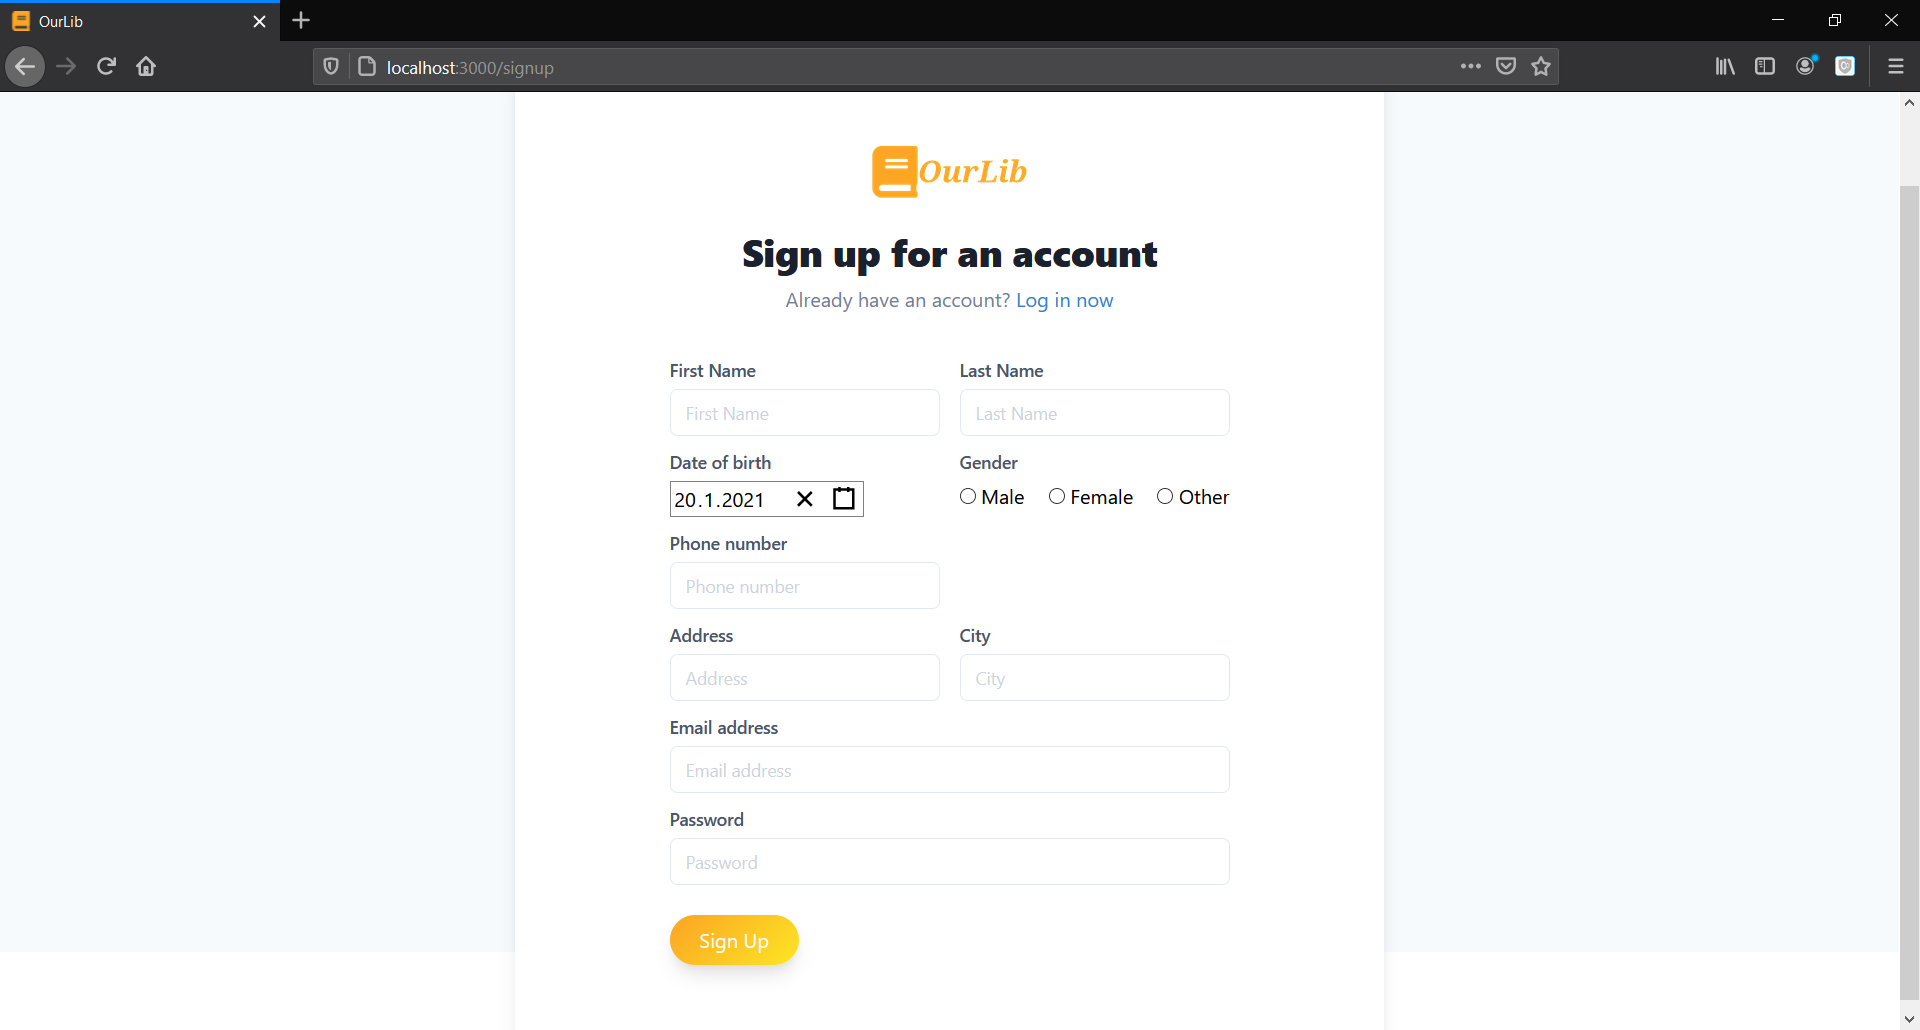
\includegraphics[width=\textwidth]{Include/Resources/FrontendScreens/React/signup.png}
    \caption{Sign up page}
    \label{fig:ScreenshotGUIsignup}
\end{figure}




%%%%%%%%%%%%%%%%%%%%%%%%%%%%%%%%%%%%%%%%%
\begin{figure}[H]
    \centering
    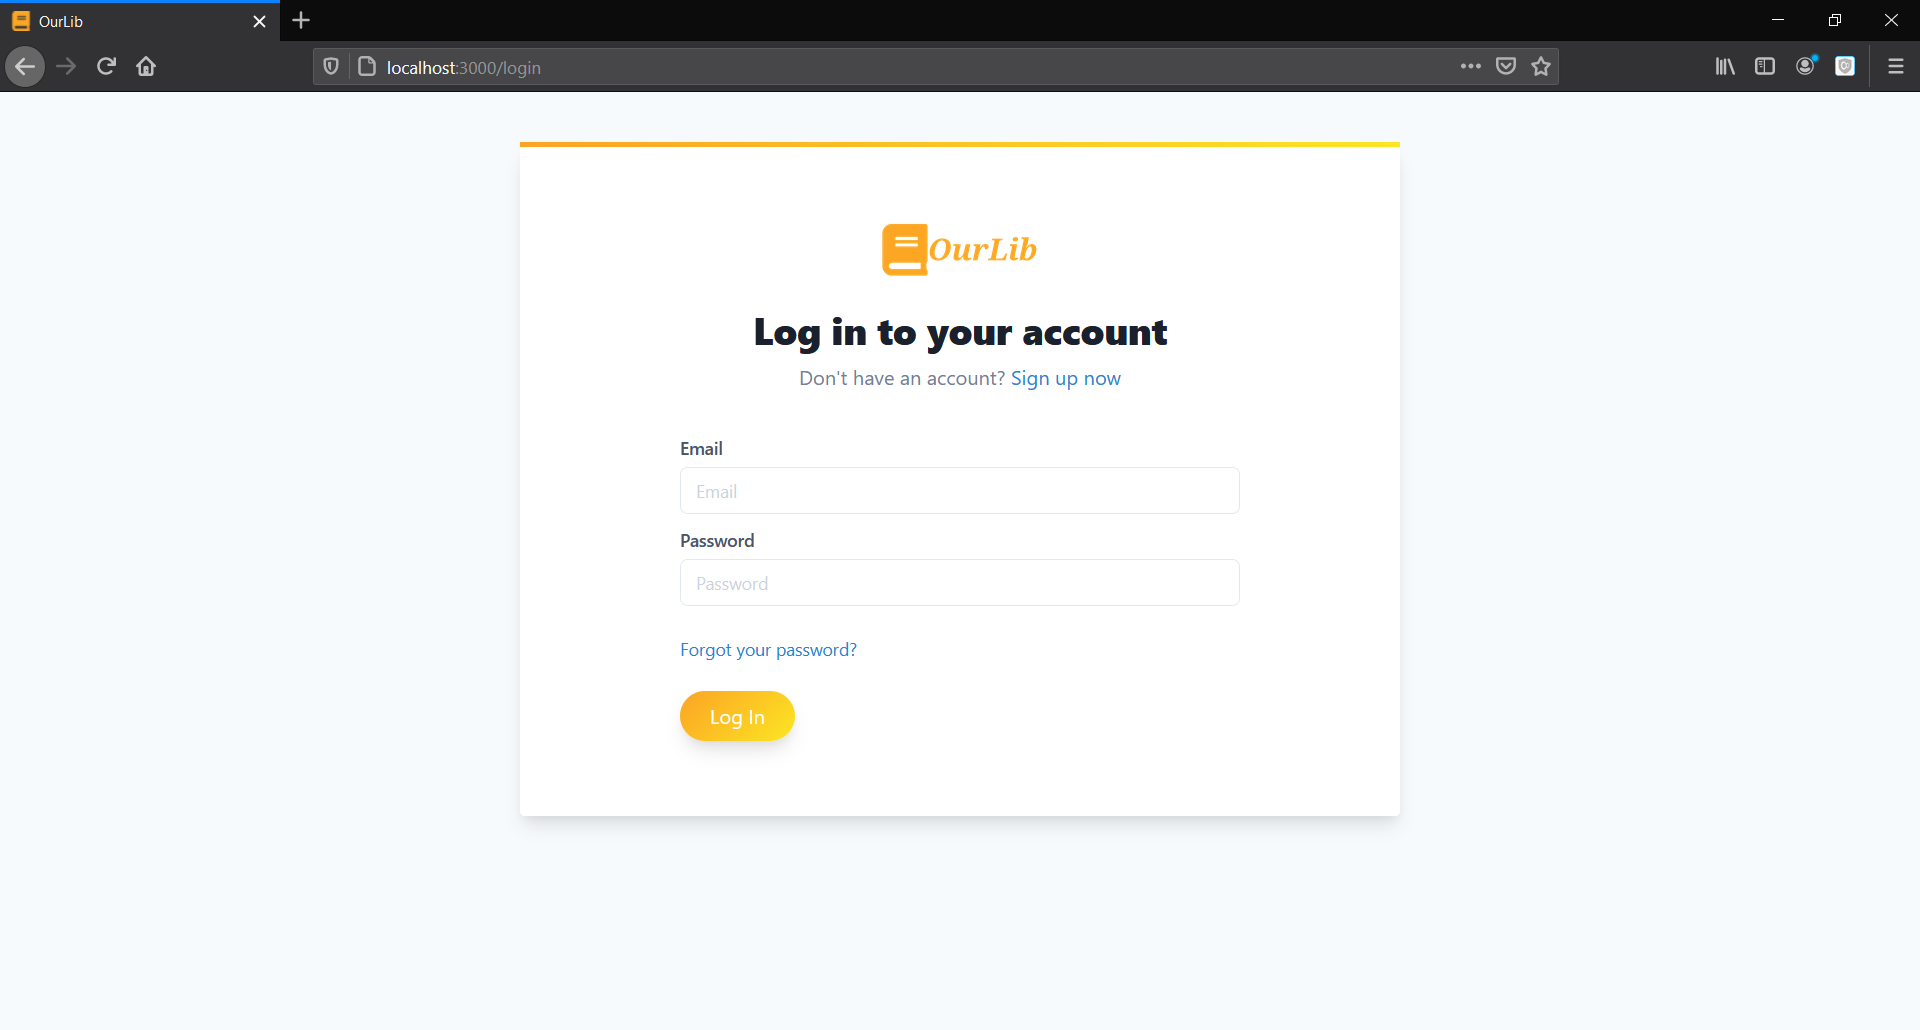
\includegraphics[width=\textwidth]{Include/Resources/FrontendScreens/React/login.png}
    \caption{Log in page}
    \label{fig:ScreenshotGUIlogin}
\end{figure}




%%%%%%%%%%%%%%%%%%%%%%%%%%%%%%%%%%%%%%%%%
\begin{figure}[H]
    \centering
    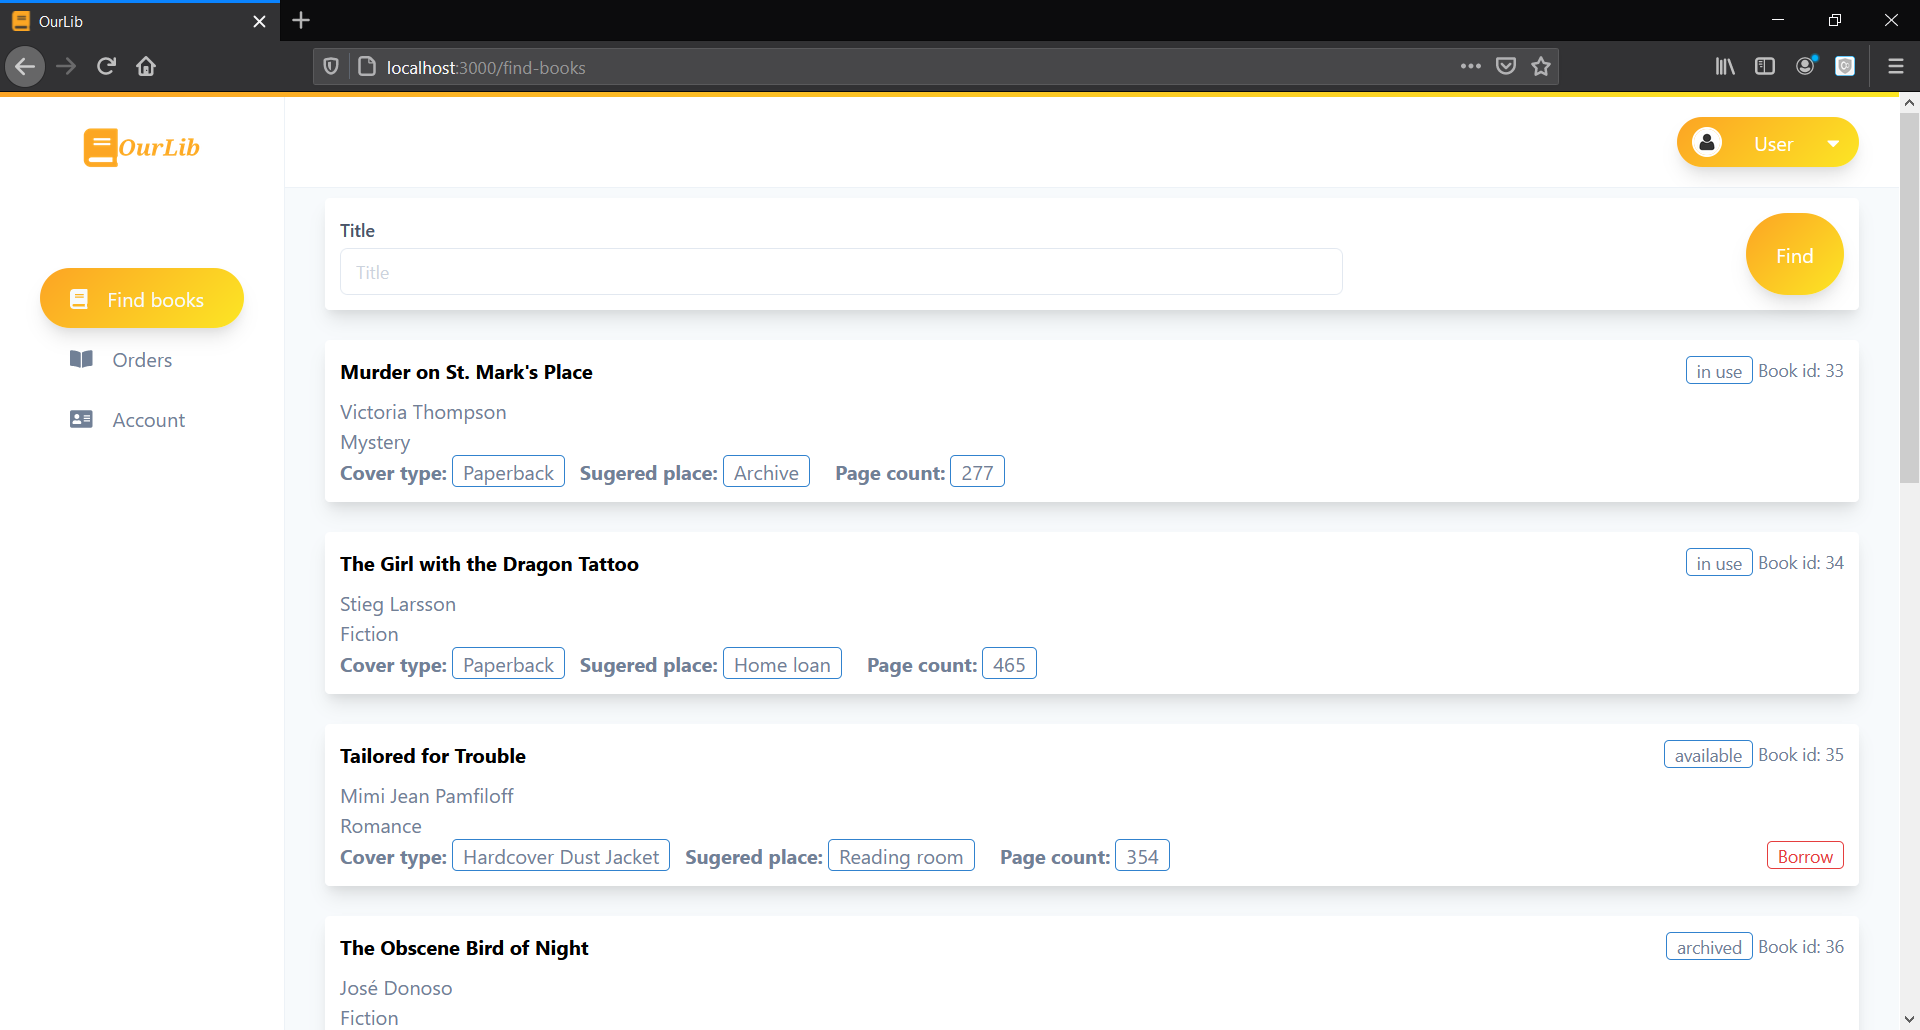
\includegraphics[width=\textwidth]{Include/Resources/FrontendScreens/React/readerFindBooks.png}
    \caption{Find books from reader account}
    \label{fig:ScreenshotGUIreaderFindBooks}
\end{figure}




%%%%%%%%%%%%%%%%%%%%%%%%%%%%%%%%%%%%%%%%%
\begin{figure}[H]
    \centering
    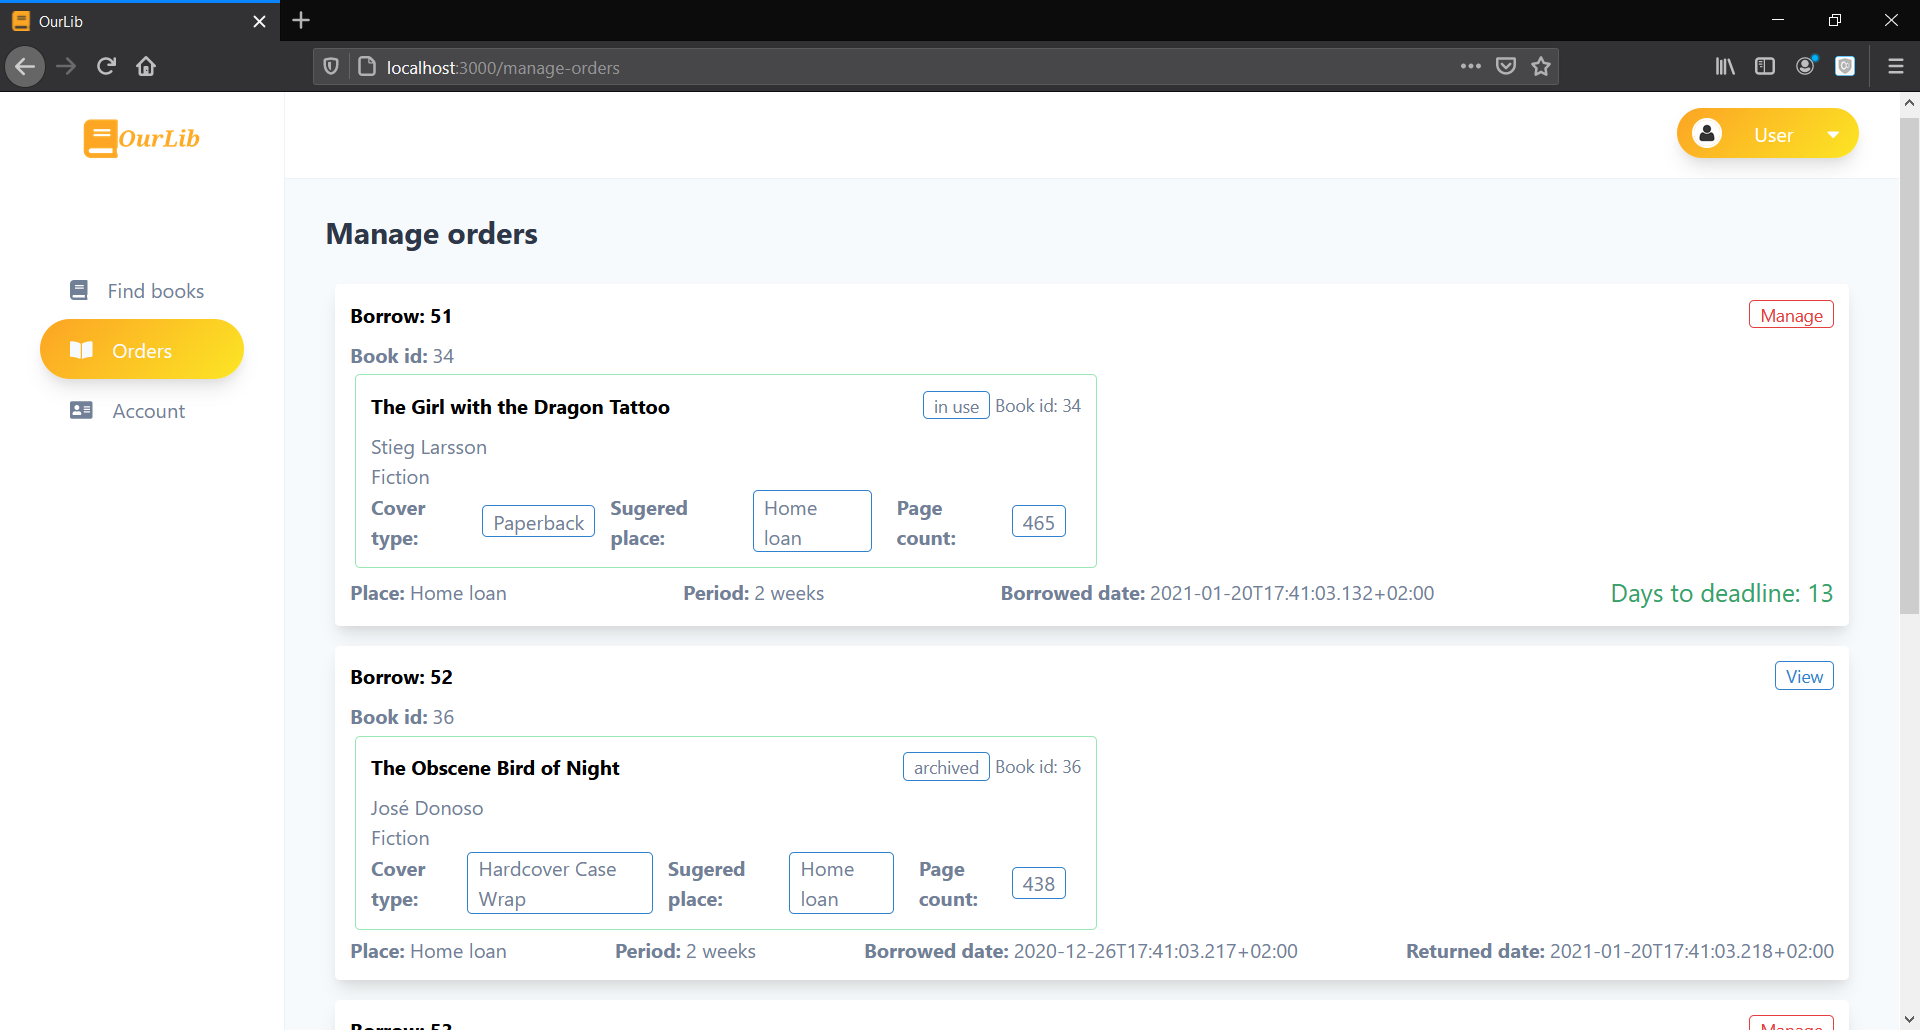
\includegraphics[width=\textwidth]{Include/Resources/FrontendScreens/React/readerOrders.png}
    \caption{Manage current reader orders}
    \label{fig:ScreenshotGUIreaderOrders}
\end{figure}




%%%%%%%%%%%%%%%%%%%%%%%%%%%%%%%%%%%%%%%%%
\begin{figure}[H]
    \centering
    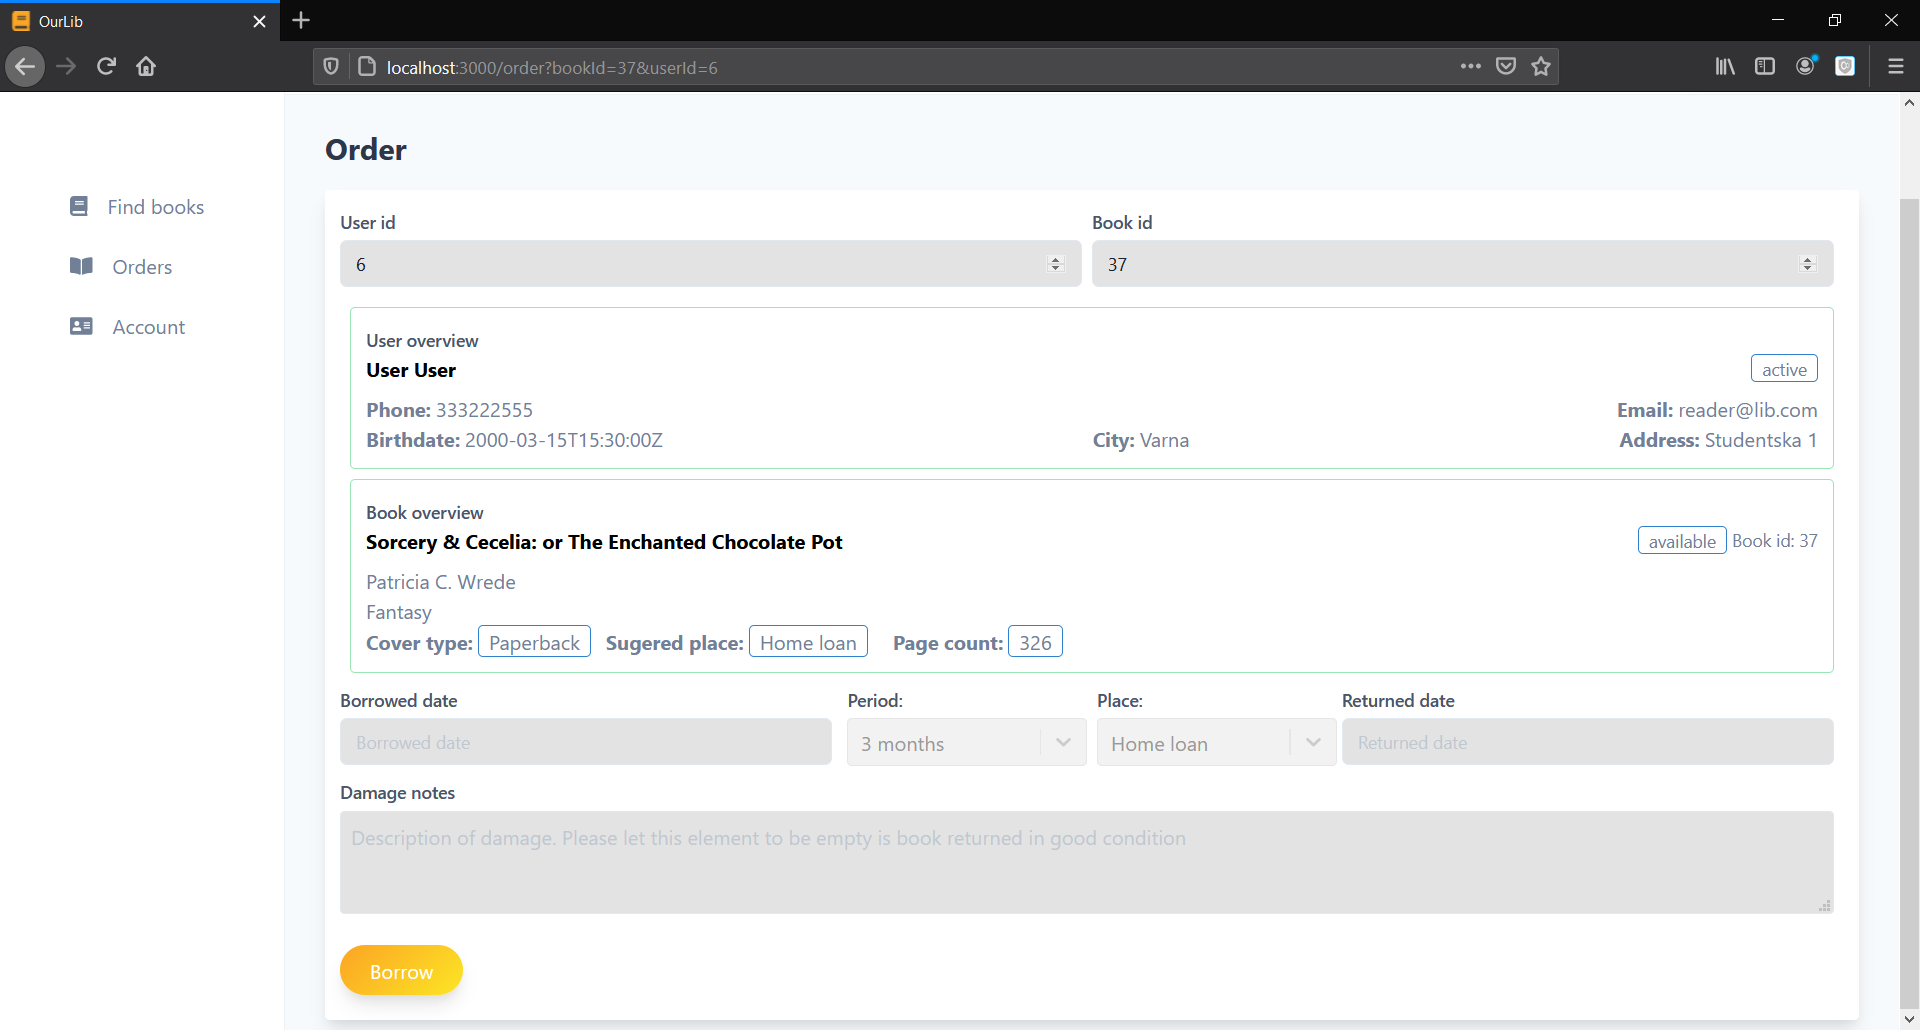
\includegraphics[width=\textwidth]{Include/Resources/FrontendScreens/React/readerBorrow.png}
    \caption{Borrow available book by reader}
    \label{fig:ScreenshotGUIreaderBorrow}
\end{figure}




%%%%%%%%%%%%%%%%%%%%%%%%%%%%%%%%%%%%%%%%%
\begin{figure}[H]
    \centering
    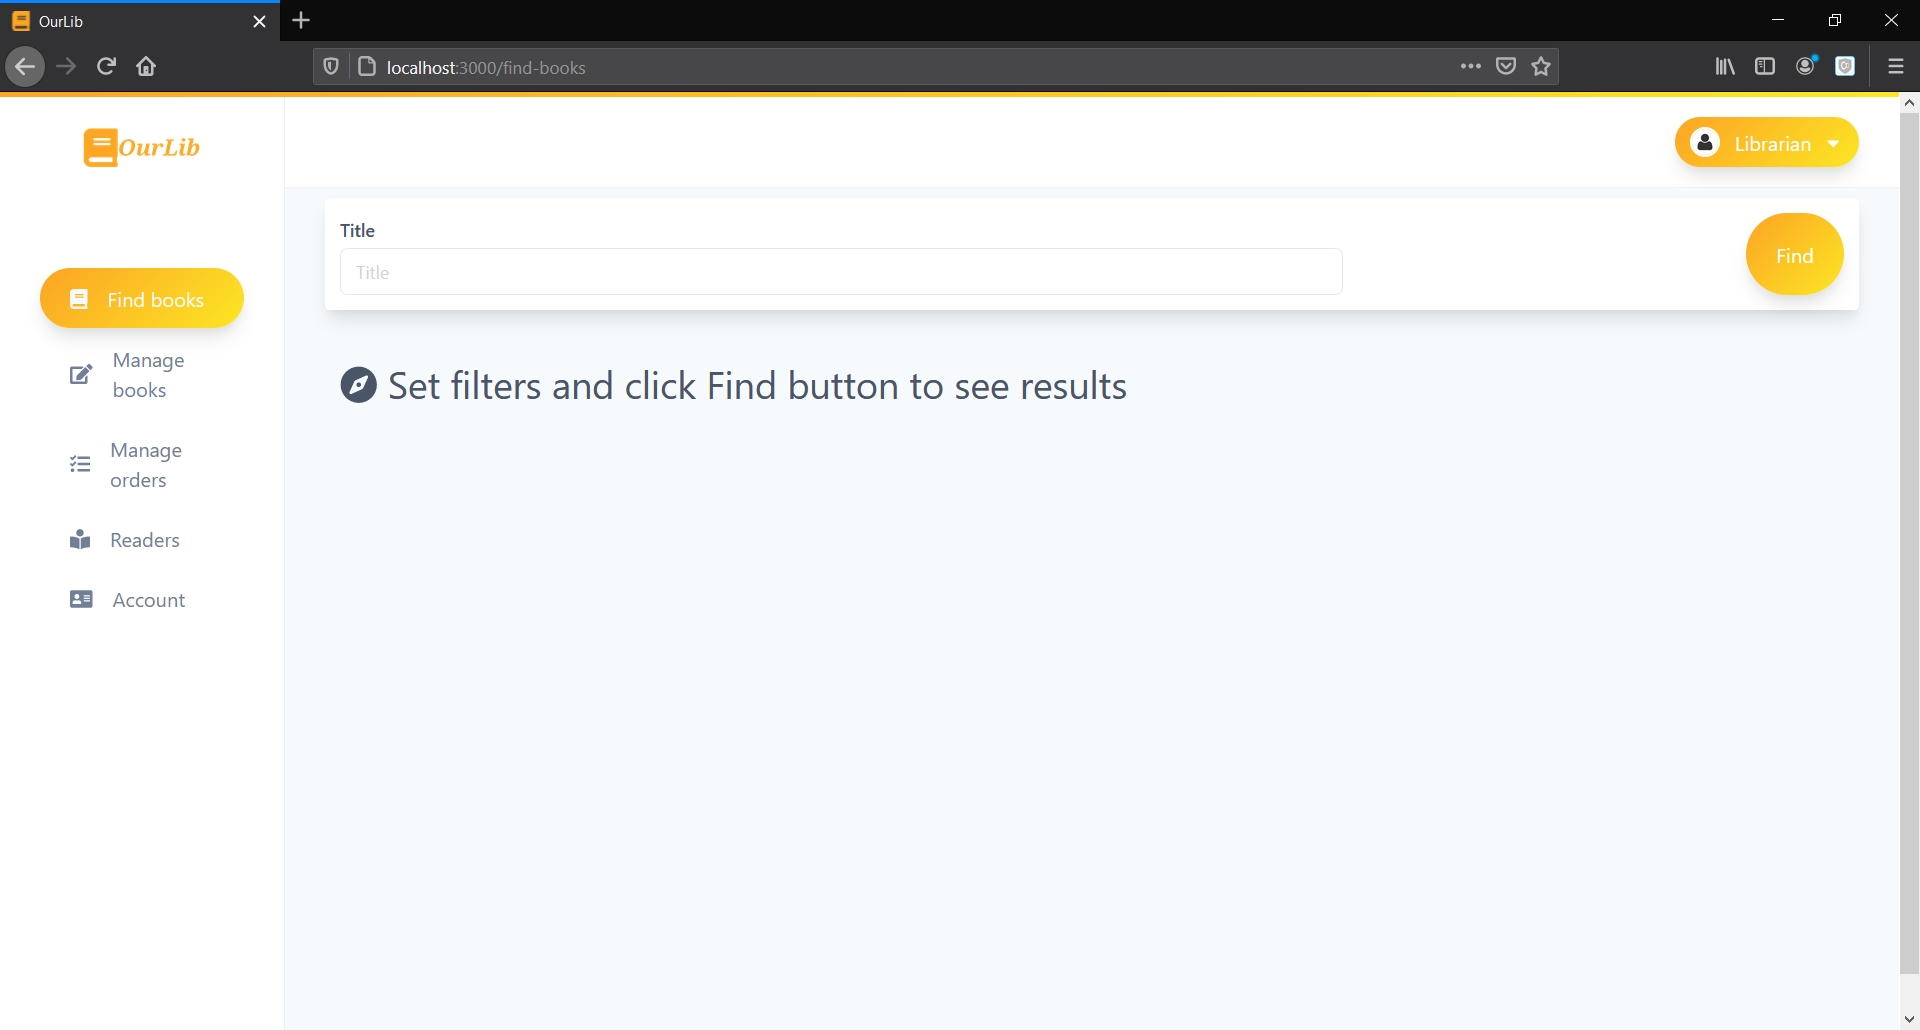
\includegraphics[width=\textwidth]{Include/Resources/FrontendScreens/React/librarianFindBooks.png}
    \caption{Find book page before find button was pressed}
    \label{fig:ScreenshotGUIlibrarianFindBooks}
\end{figure}




%%%%%%%%%%%%%%%%%%%%%%%%%%%%%%%%%%%%%%%%%
\begin{figure}[H]
    \centering
    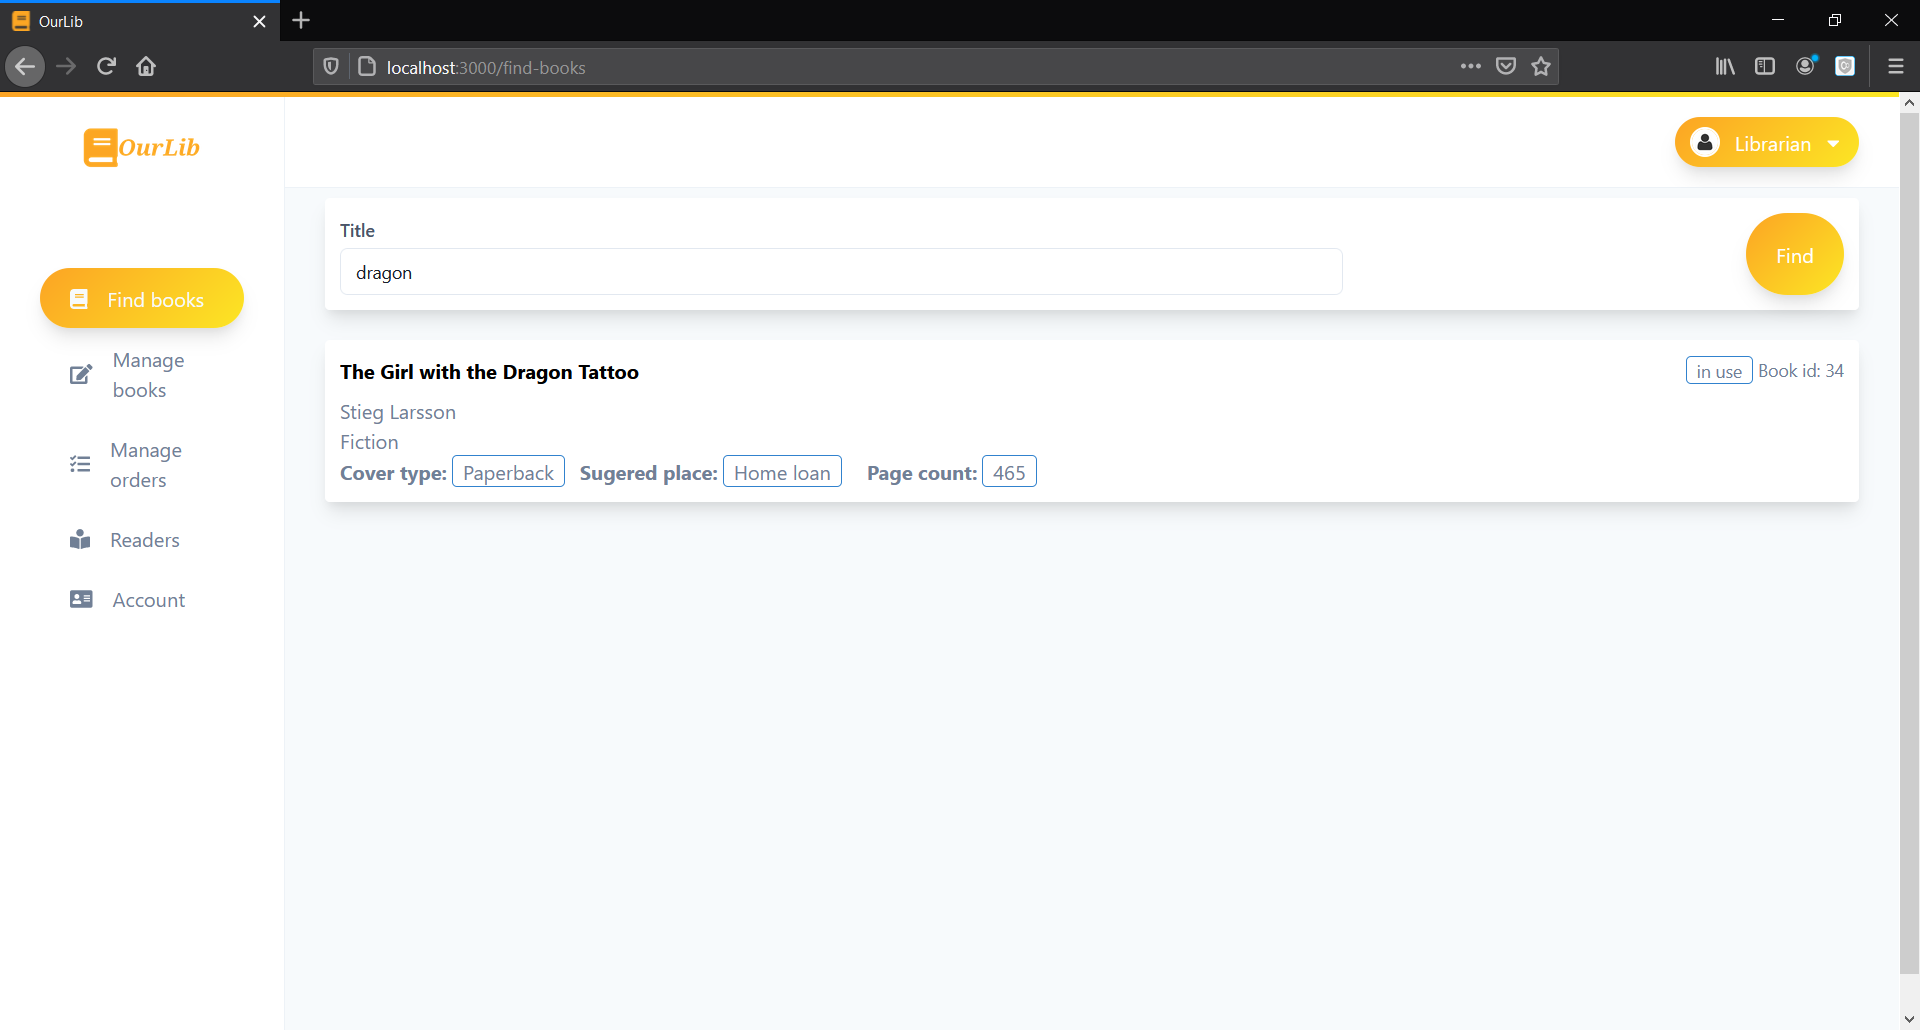
\includegraphics[width=\textwidth]{Include/Resources/FrontendScreens/React/librarianFindBooks2.png}
    \caption{Searching phrase in search bar}
    \label{fig:ScreenshotGUIlibrarianFindBooks2}
\end{figure}




%%%%%%%%%%%%%%%%%%%%%%%%%%%%%%%%%%%%%%%%%
\begin{figure}[H]
    \centering
    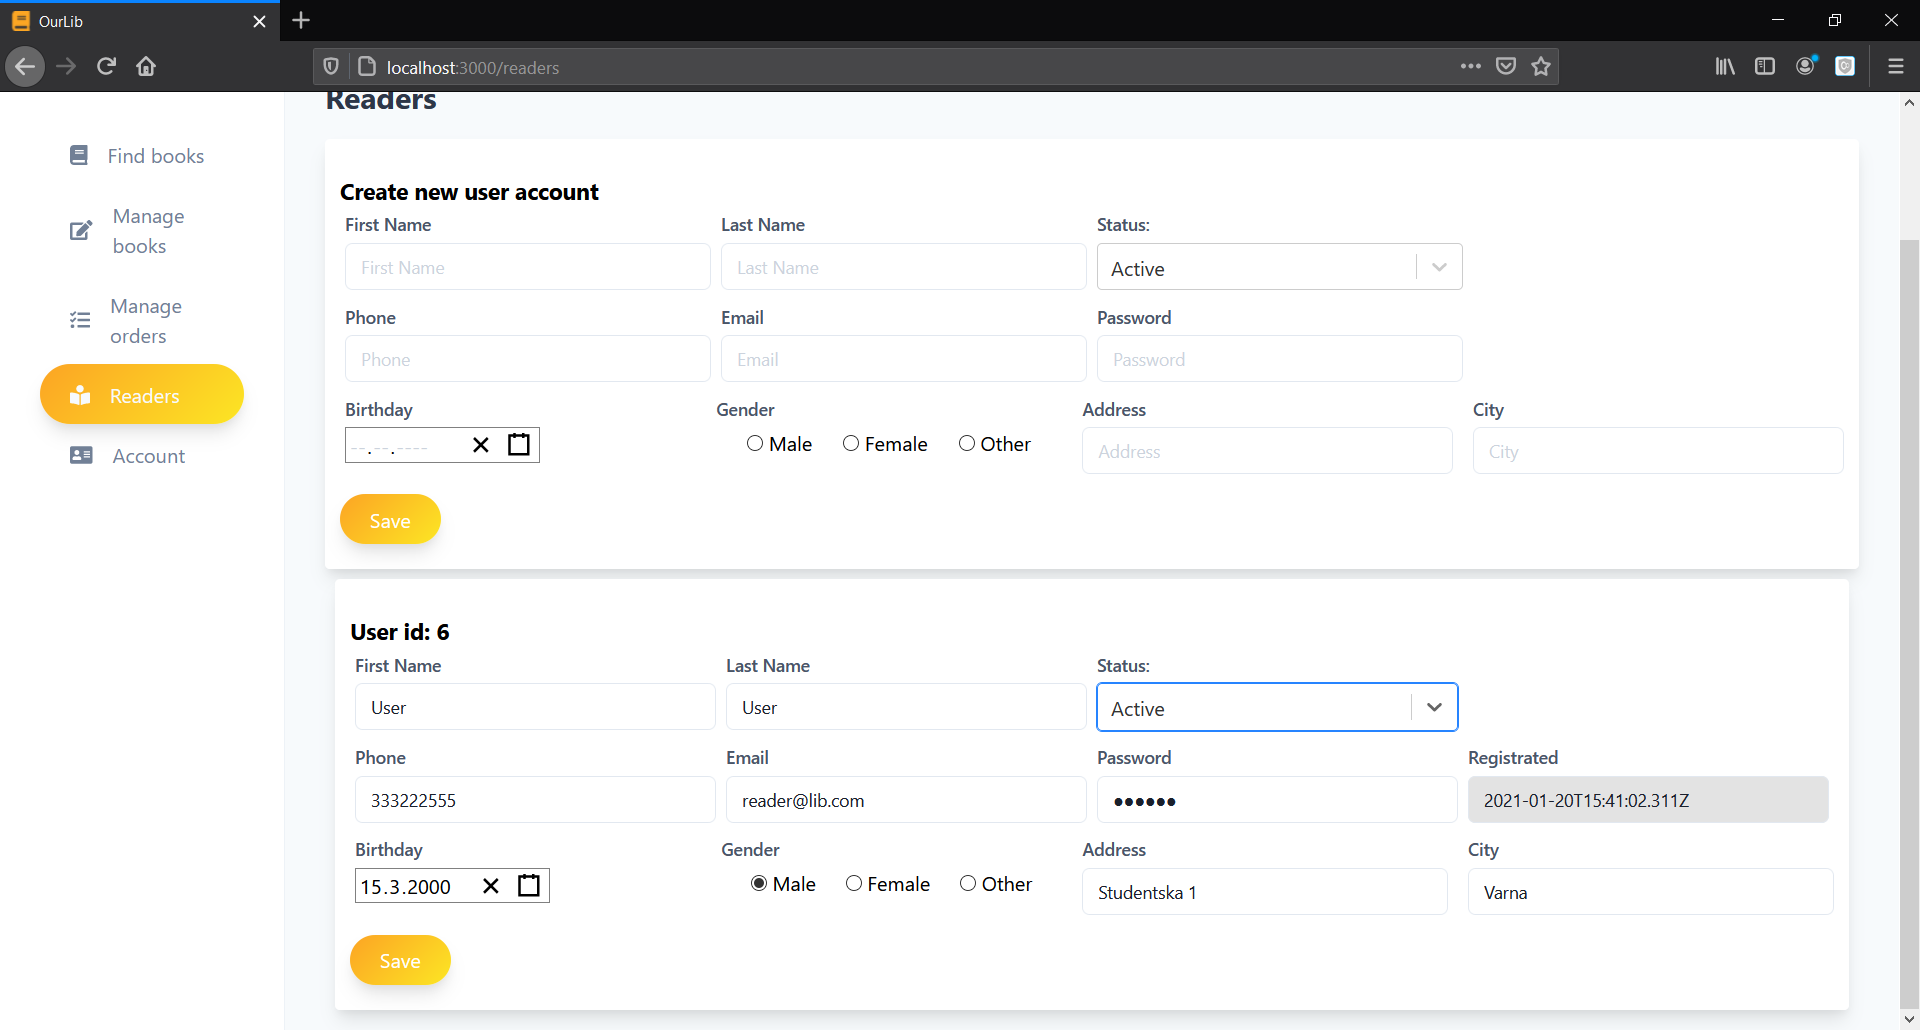
\includegraphics[width=\textwidth]{Include/Resources/FrontendScreens/React/librarianReaders.png}
    \caption{Manage all readers available in system}
    \label{fig:ScreenshotGUIlibrarianReaders}
\end{figure}




%%%%%%%%%%%%%%%%%%%%%%%%%%%%%%%%%%%%%%%%%
\begin{figure}[H]
    \centering
    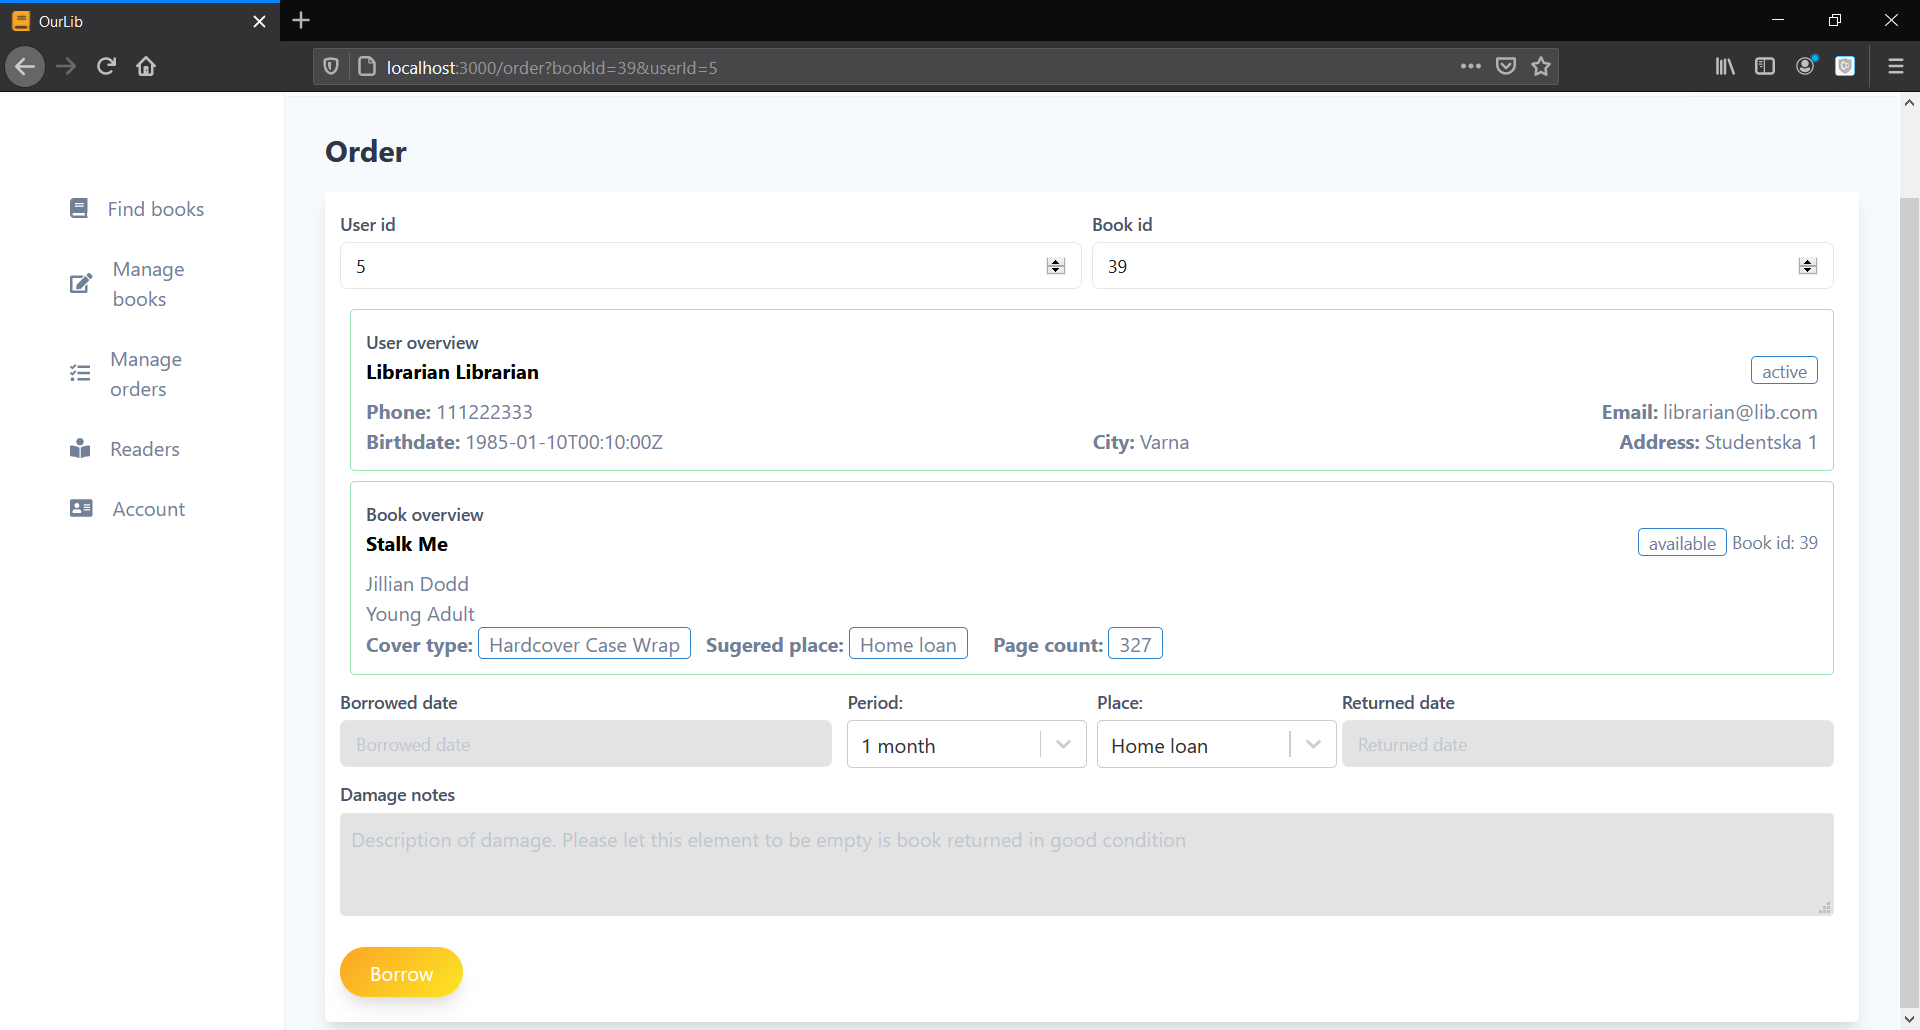
\includegraphics[width=\textwidth]{Include/Resources/FrontendScreens/React/librarianBorrow.png}
    \caption{Borrow any available book for any reader}
    \label{fig:ScreenshotGUIlibrarianBorrow}
\end{figure}




%%%%%%%%%%%%%%%%%%%%%%%%%%%%%%%%%%%%%%%%%
\begin{figure}[H]
    \centering
    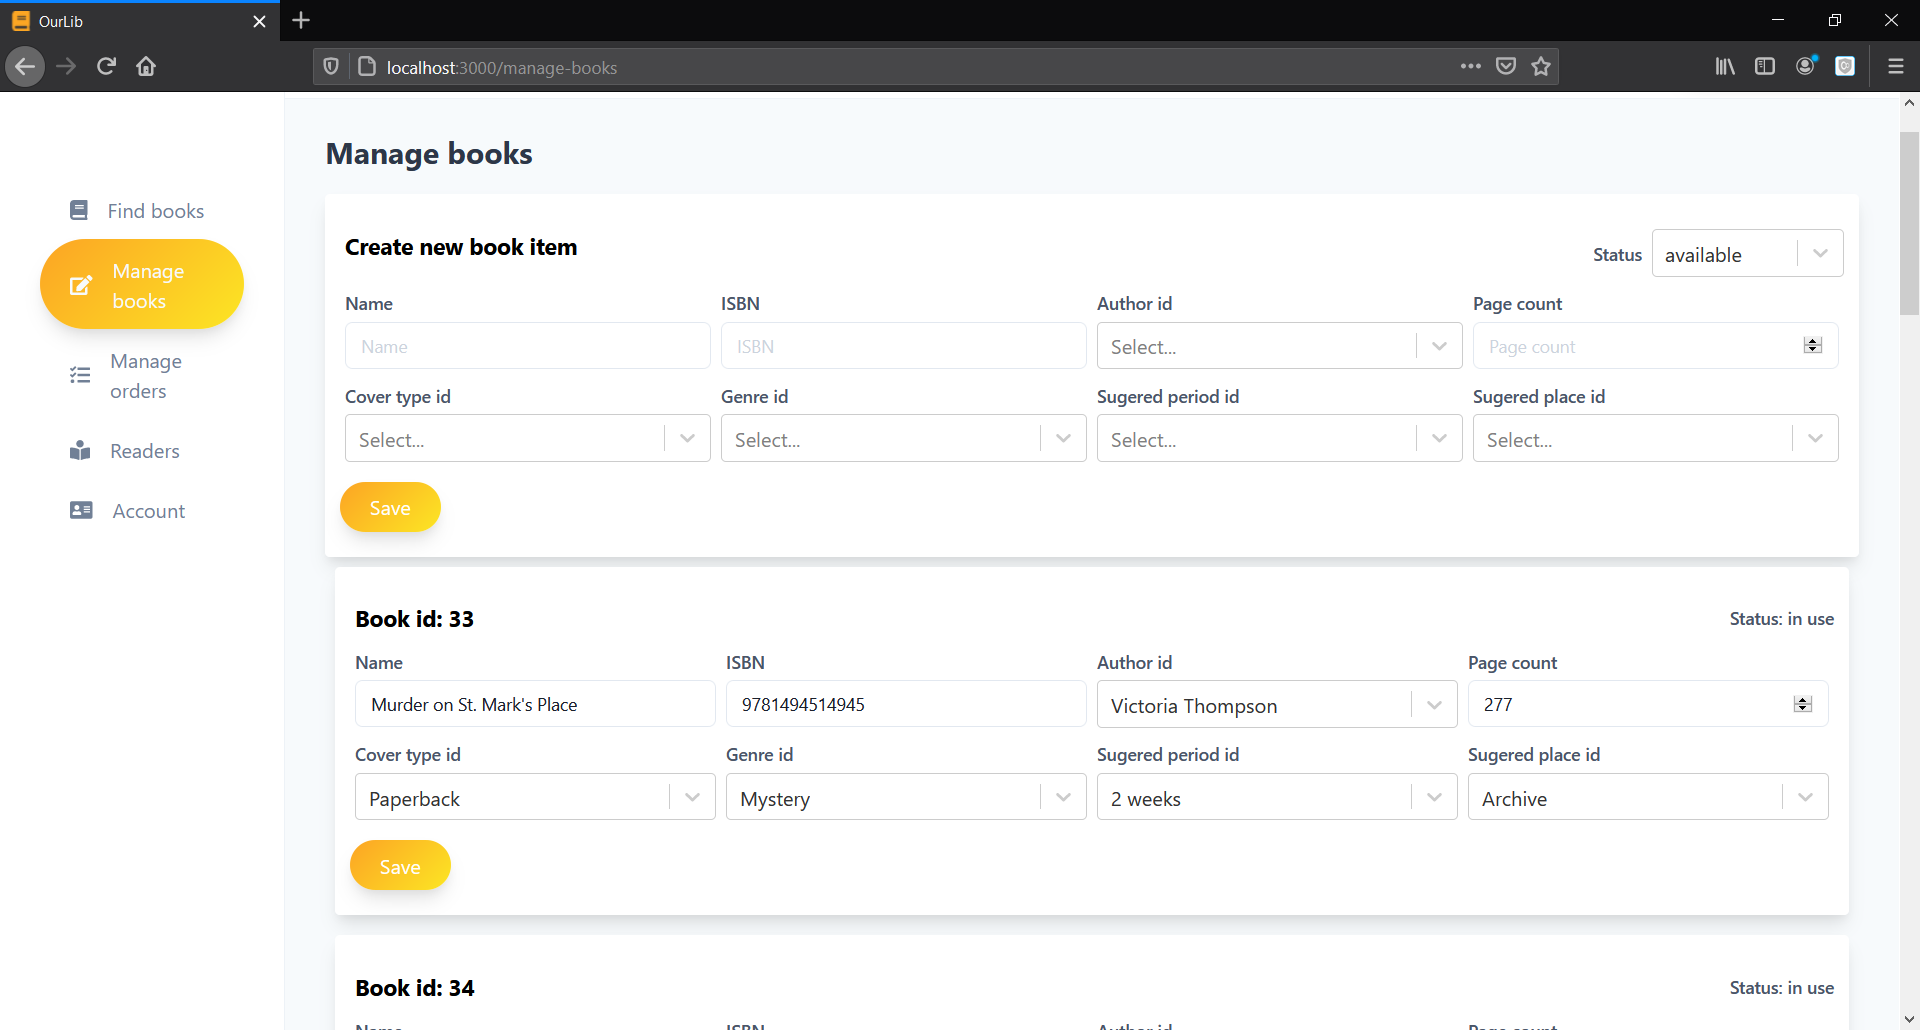
\includegraphics[width=\textwidth]{Include/Resources/FrontendScreens/React/librarianManageBooks.png}
    \caption{Manage all books in system}
    \label{fig:ScreenshotGUIlibrarianManageBooks}
\end{figure}




%%%%%%%%%%%%%%%%%%%%%%%%%%%%%%%%%%%%%%%%%
\begin{figure}[H]
    \centering
    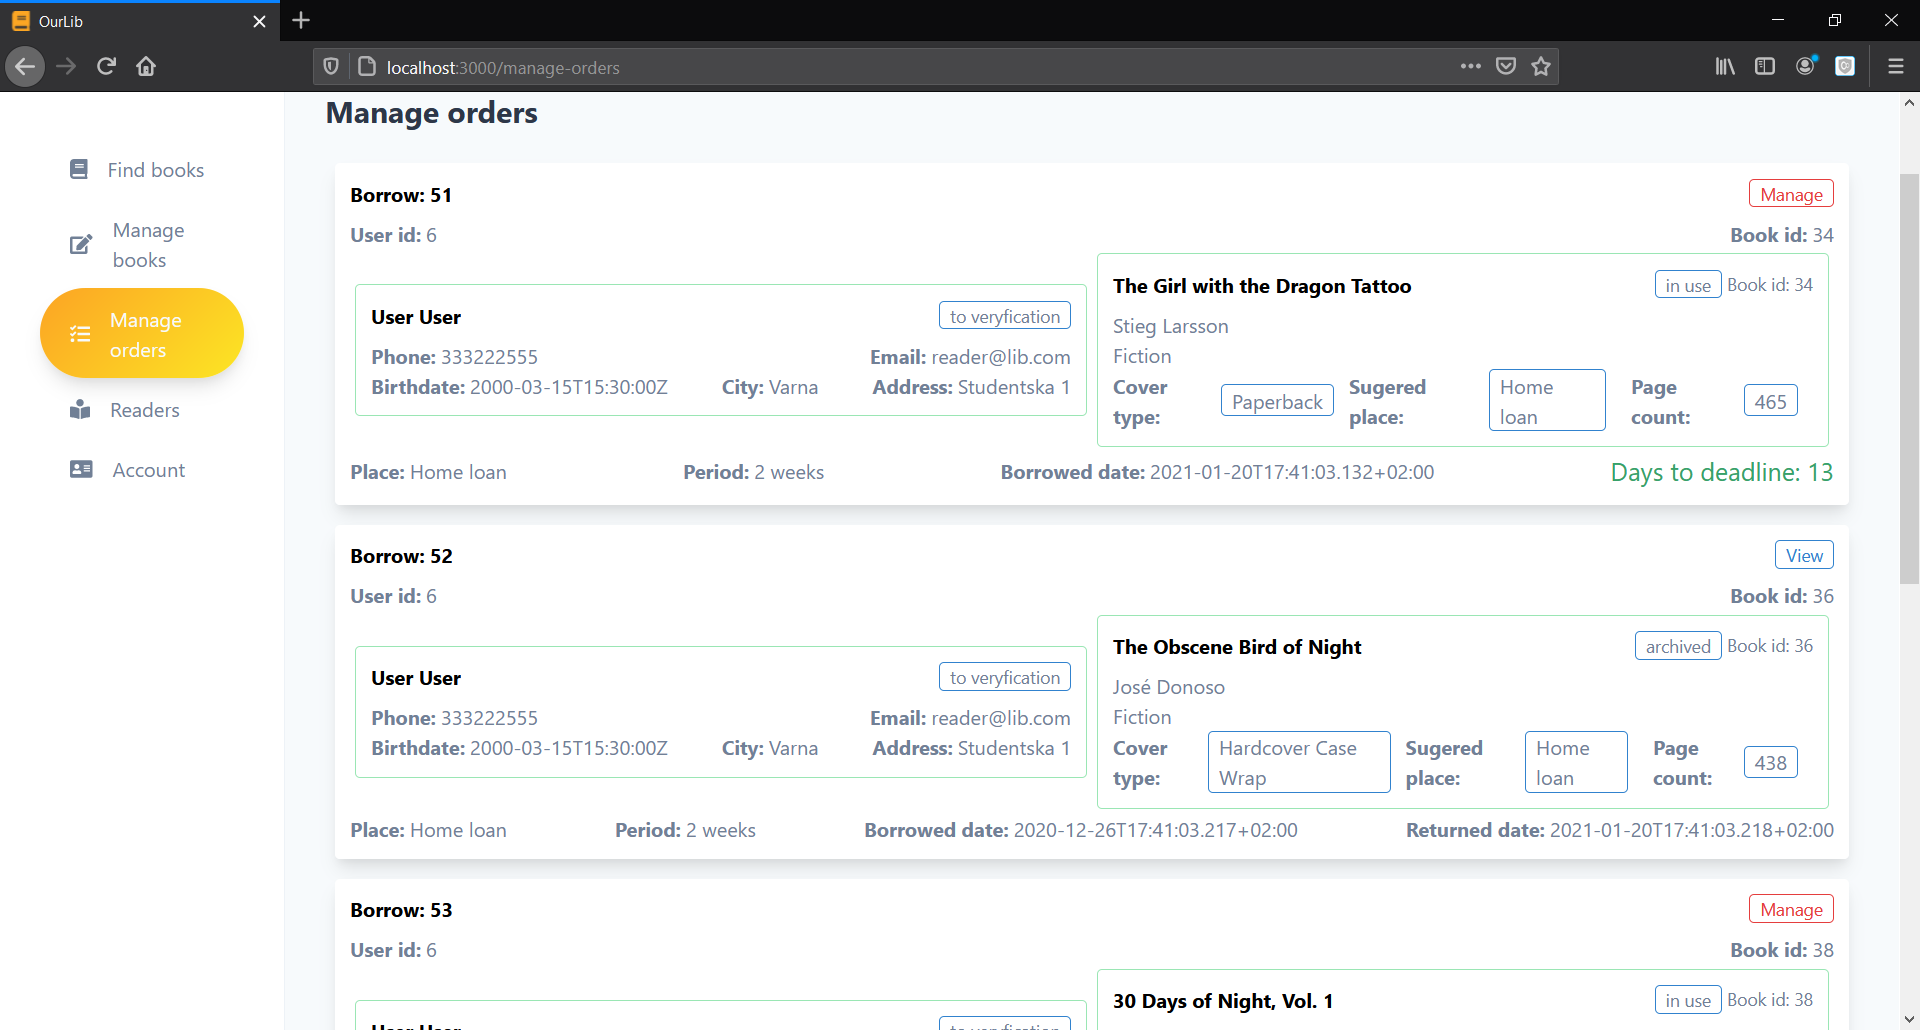
\includegraphics[width=\textwidth]{Include/Resources/FrontendScreens/React/librarianManageOrders.png}
    \caption{Manage all orders in system}
    \label{fig:ScreenshotGUIlibrarianManageOrders}
\end{figure}




%%%%%%%%%%%%%%%%%%%%%%%%%%%%%%%%%%%%%%%%%
\begin{figure}[H]
    \centering
    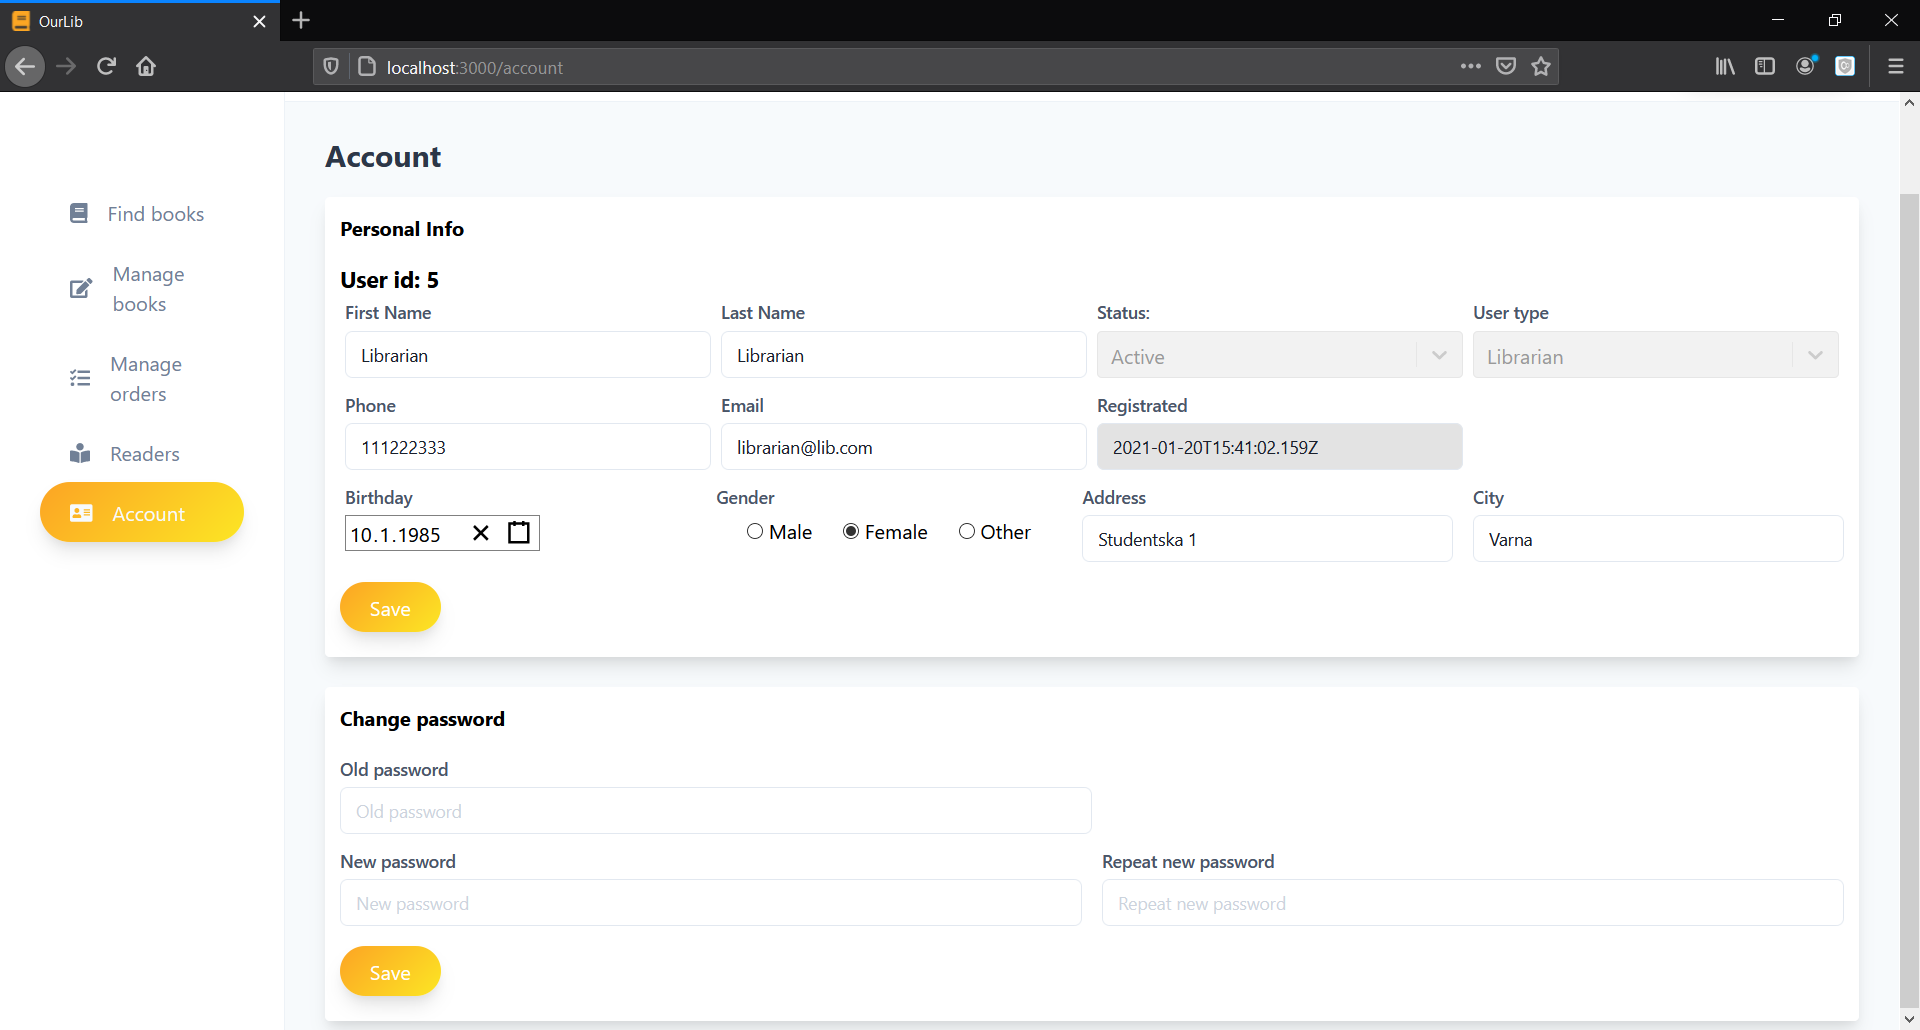
\includegraphics[width=\textwidth]{Include/Resources/FrontendScreens/React/librarianAccount.png}
    \caption{Change credentials of current user}
    \label{fig:ScreenshotGUIlibrarianAccount}
\end{figure}




%%%%%%%%%%%%%%%%%%%%%%%%%%%%%%%%%%%%%%%%%
\begin{figure}[H]
    \centering
    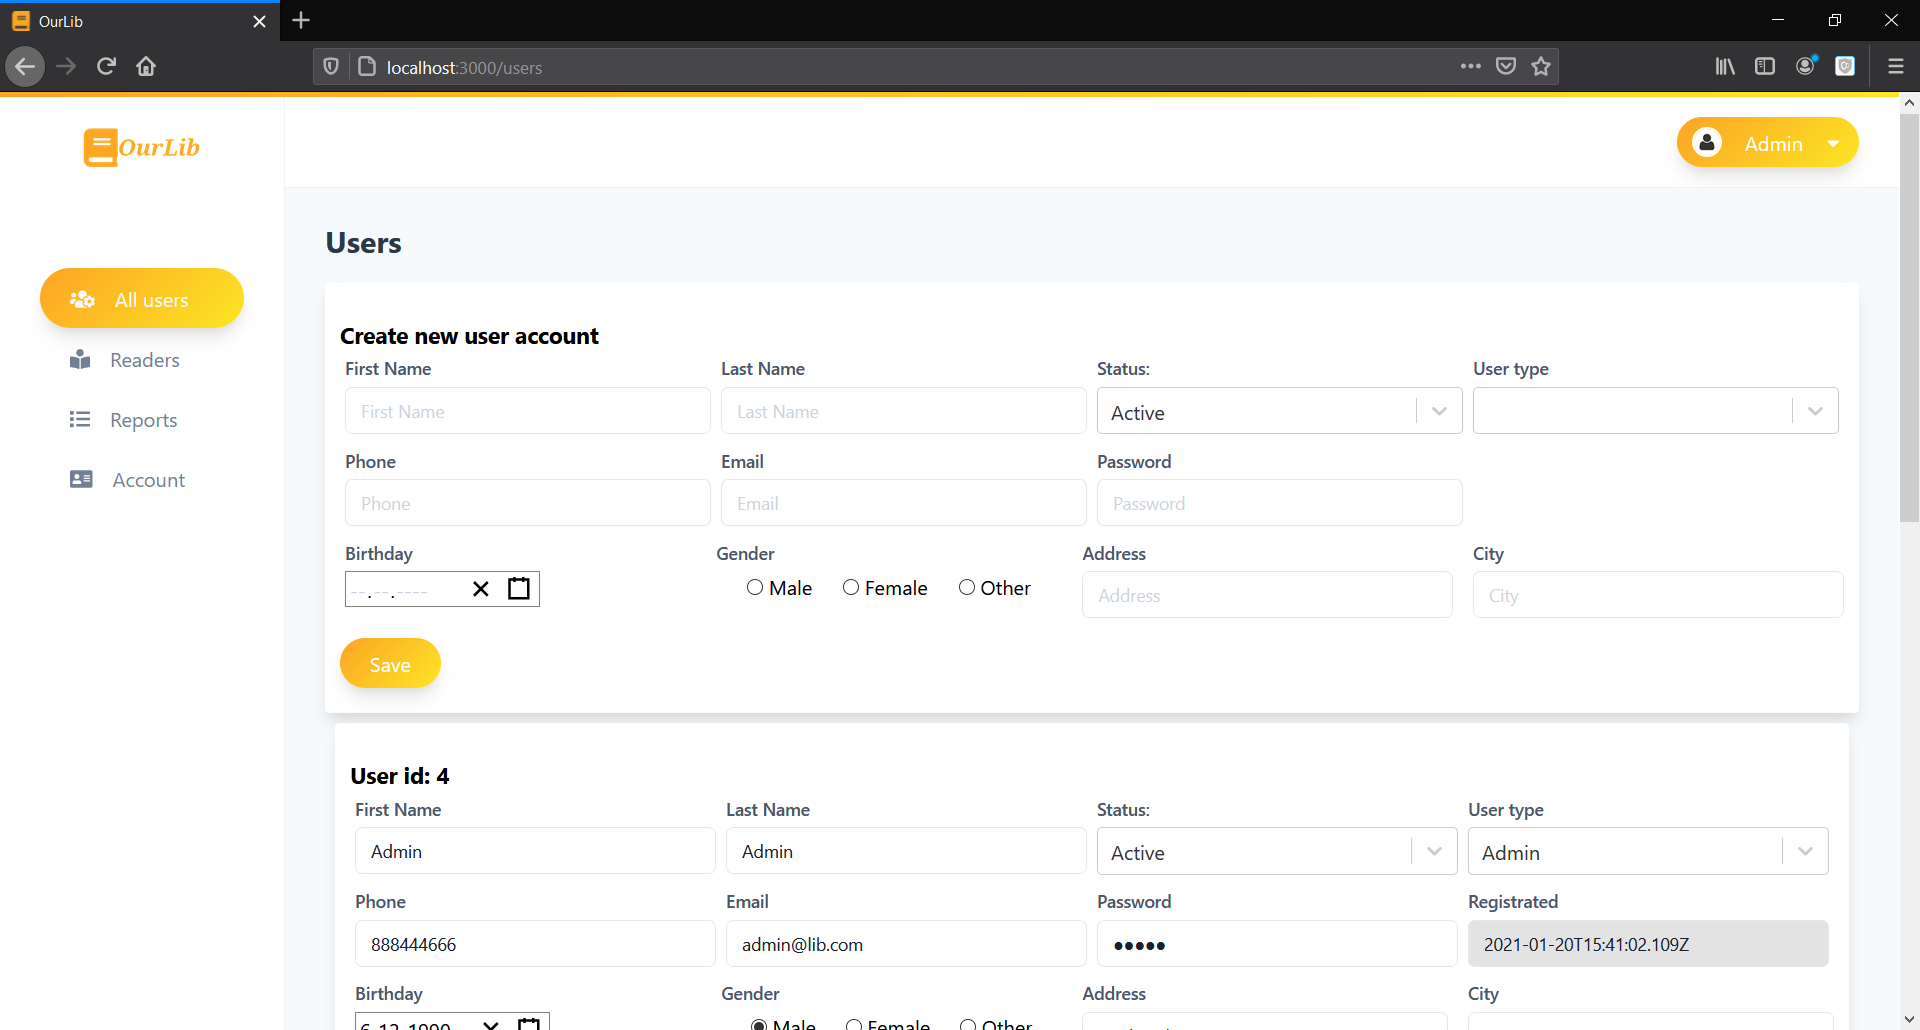
\includegraphics[width=\textwidth]{Include/Resources/FrontendScreens/React/adminUsers.png}
    \caption{Manage all users in system}
    \label{fig:ScreenshotGUIadminUsers}
\end{figure}




%%%%%%%%%%%%%%%%%%%%%%%%%%%%%%%%%%%%%%%%%
\begin{figure}[H]
    \centering
    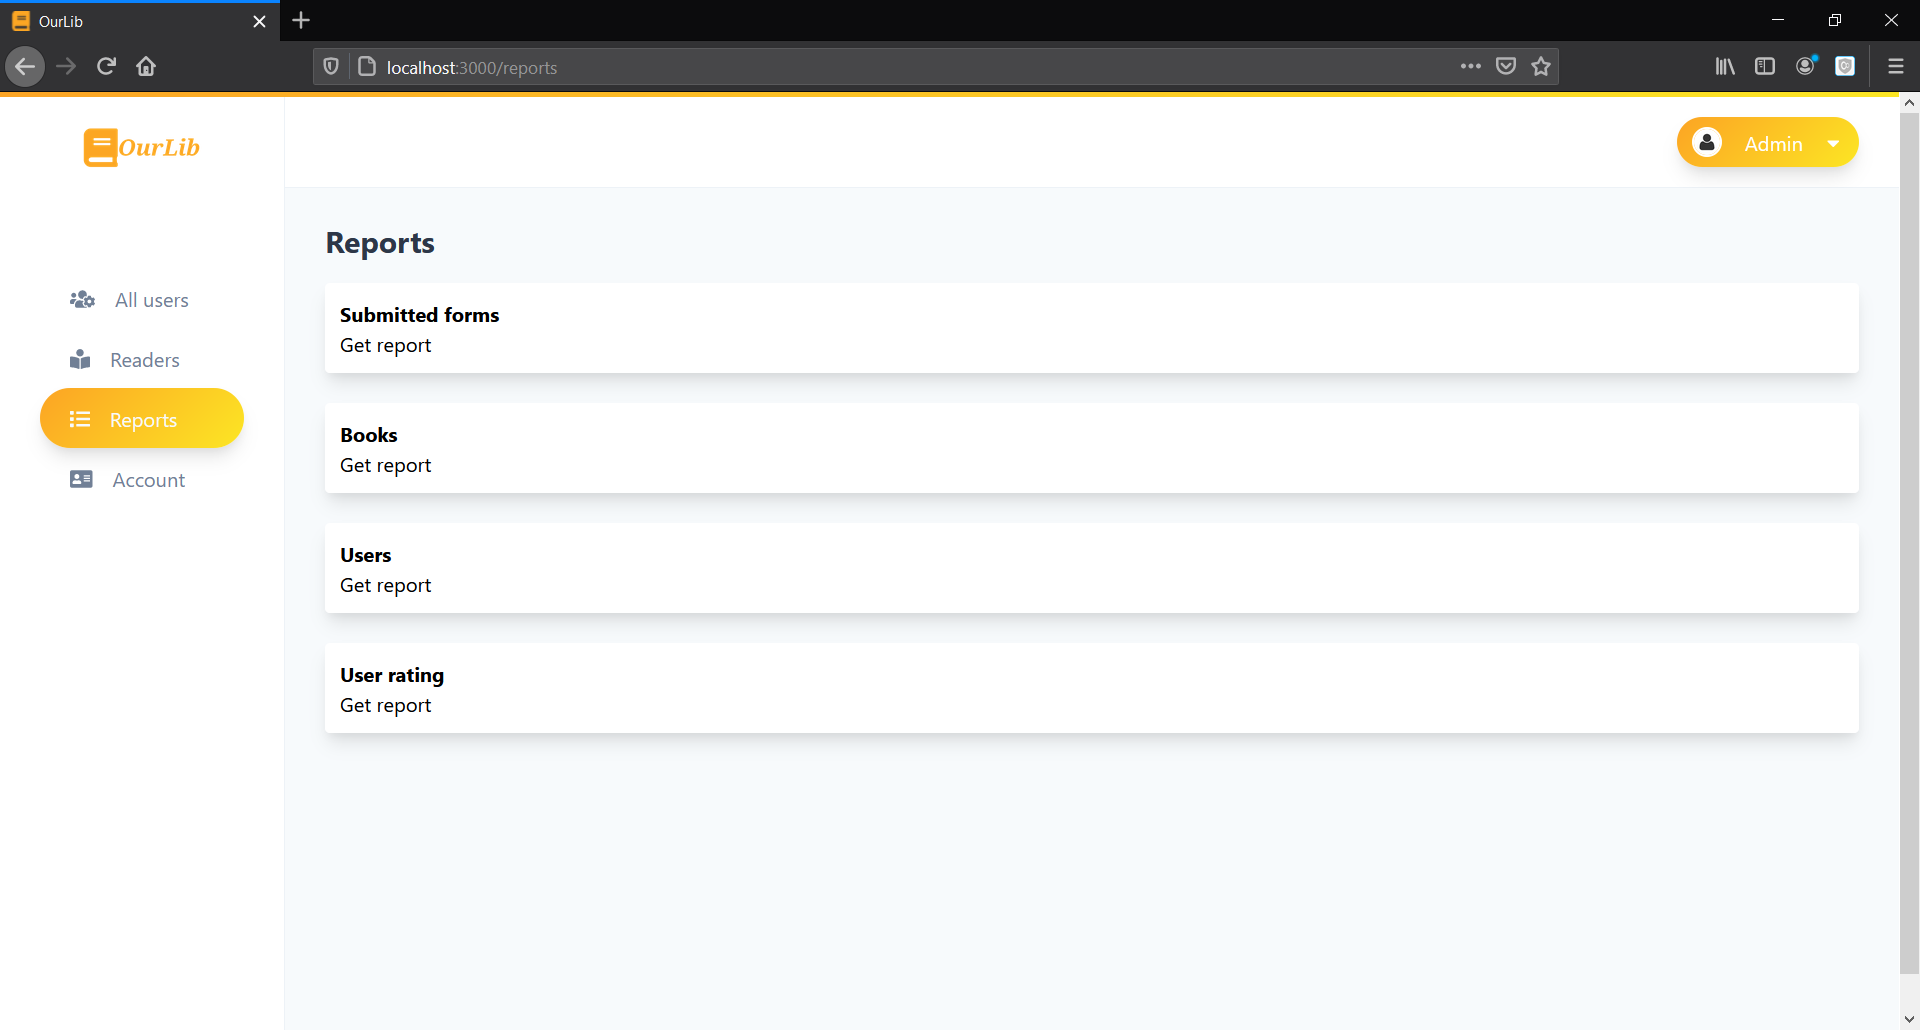
\includegraphics[width=\textwidth]{Include/Resources/FrontendScreens/React/adminReports.png}
    \caption{Reports main navigation page}
    \label{fig:ScreenshotGUIadminReports}
\end{figure}




%%%%%%%%%%%%%%%%%%%%%%%%%%%%%%%%%%%%%%%%%
\begin{figure}[H]
    \centering
    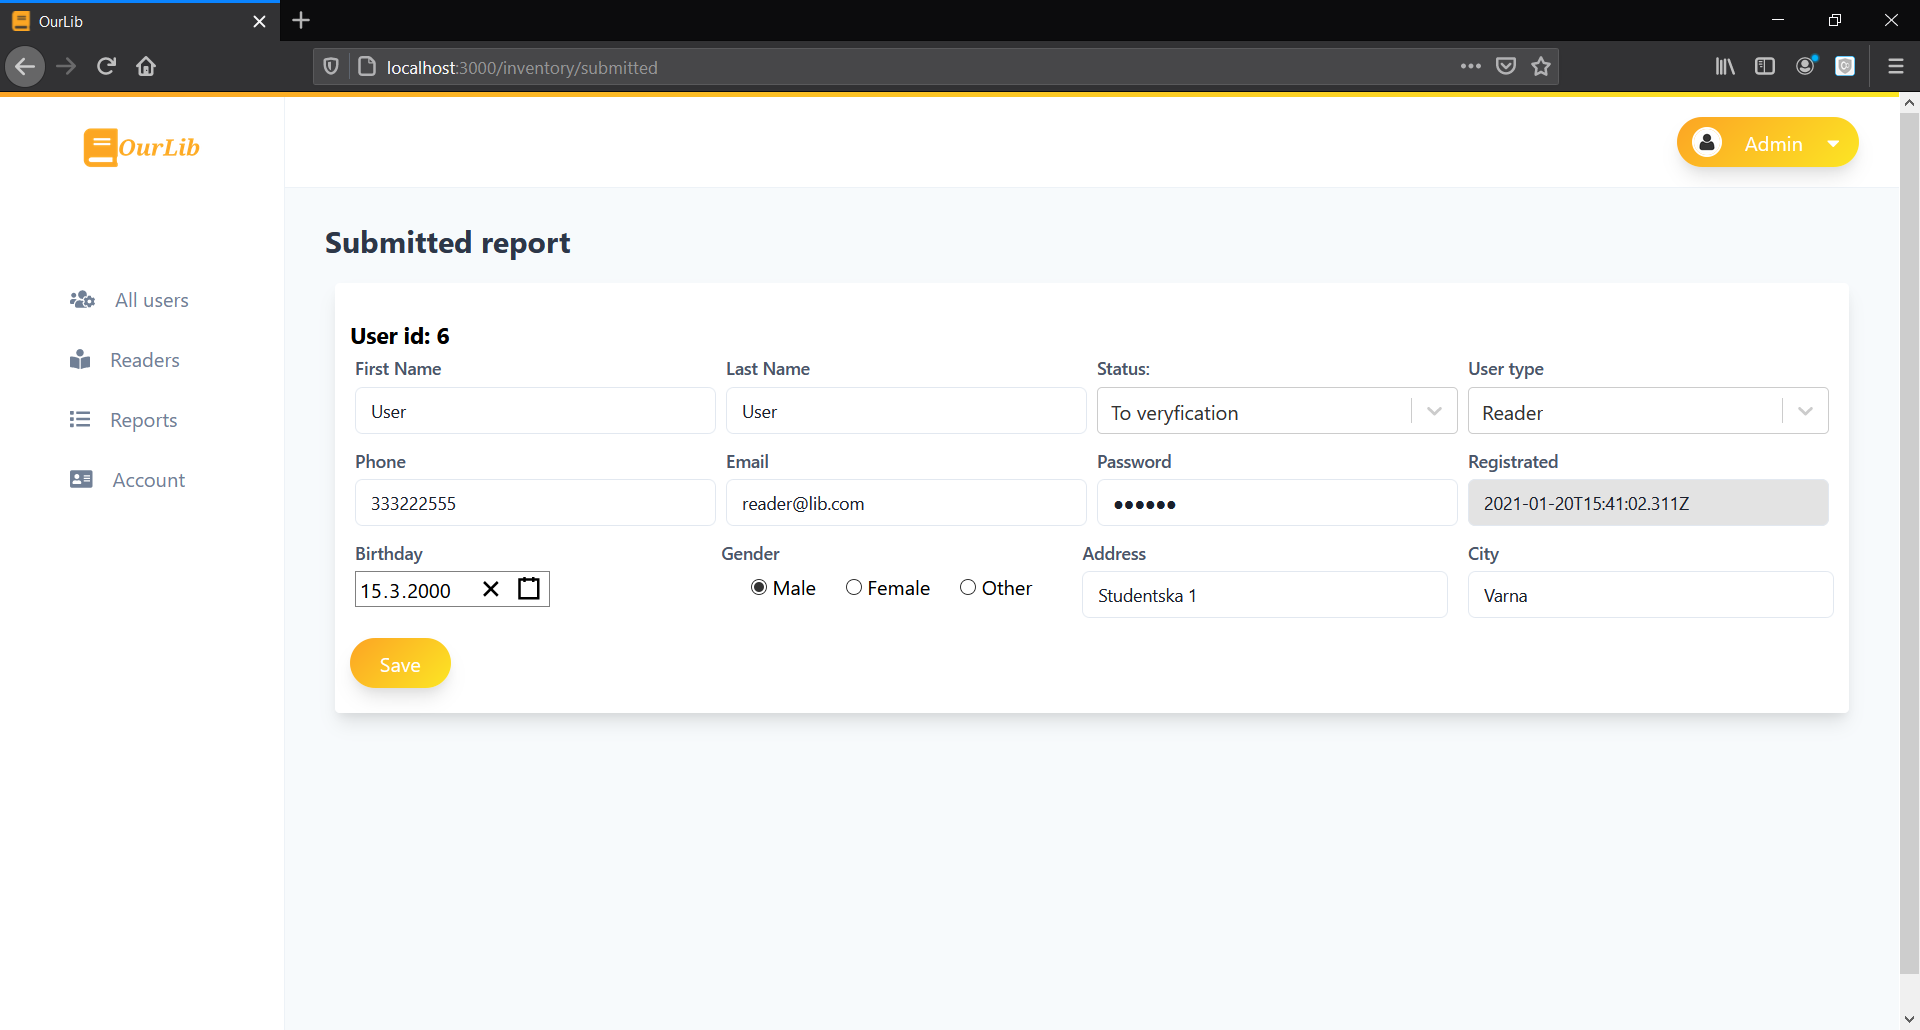
\includegraphics[width=\textwidth]{Include/Resources/FrontendScreens/React/adminSubmittedReport.png}
    \caption{Manage new submitted readers}
    \label{fig:ScreenshotGUIadminSubmittedReport}
\end{figure}




%%%%%%%%%%%%%%%%%%%%%%%%%%%%%%%%%%%%%%%%%
\begin{figure}[H]
    \centering
    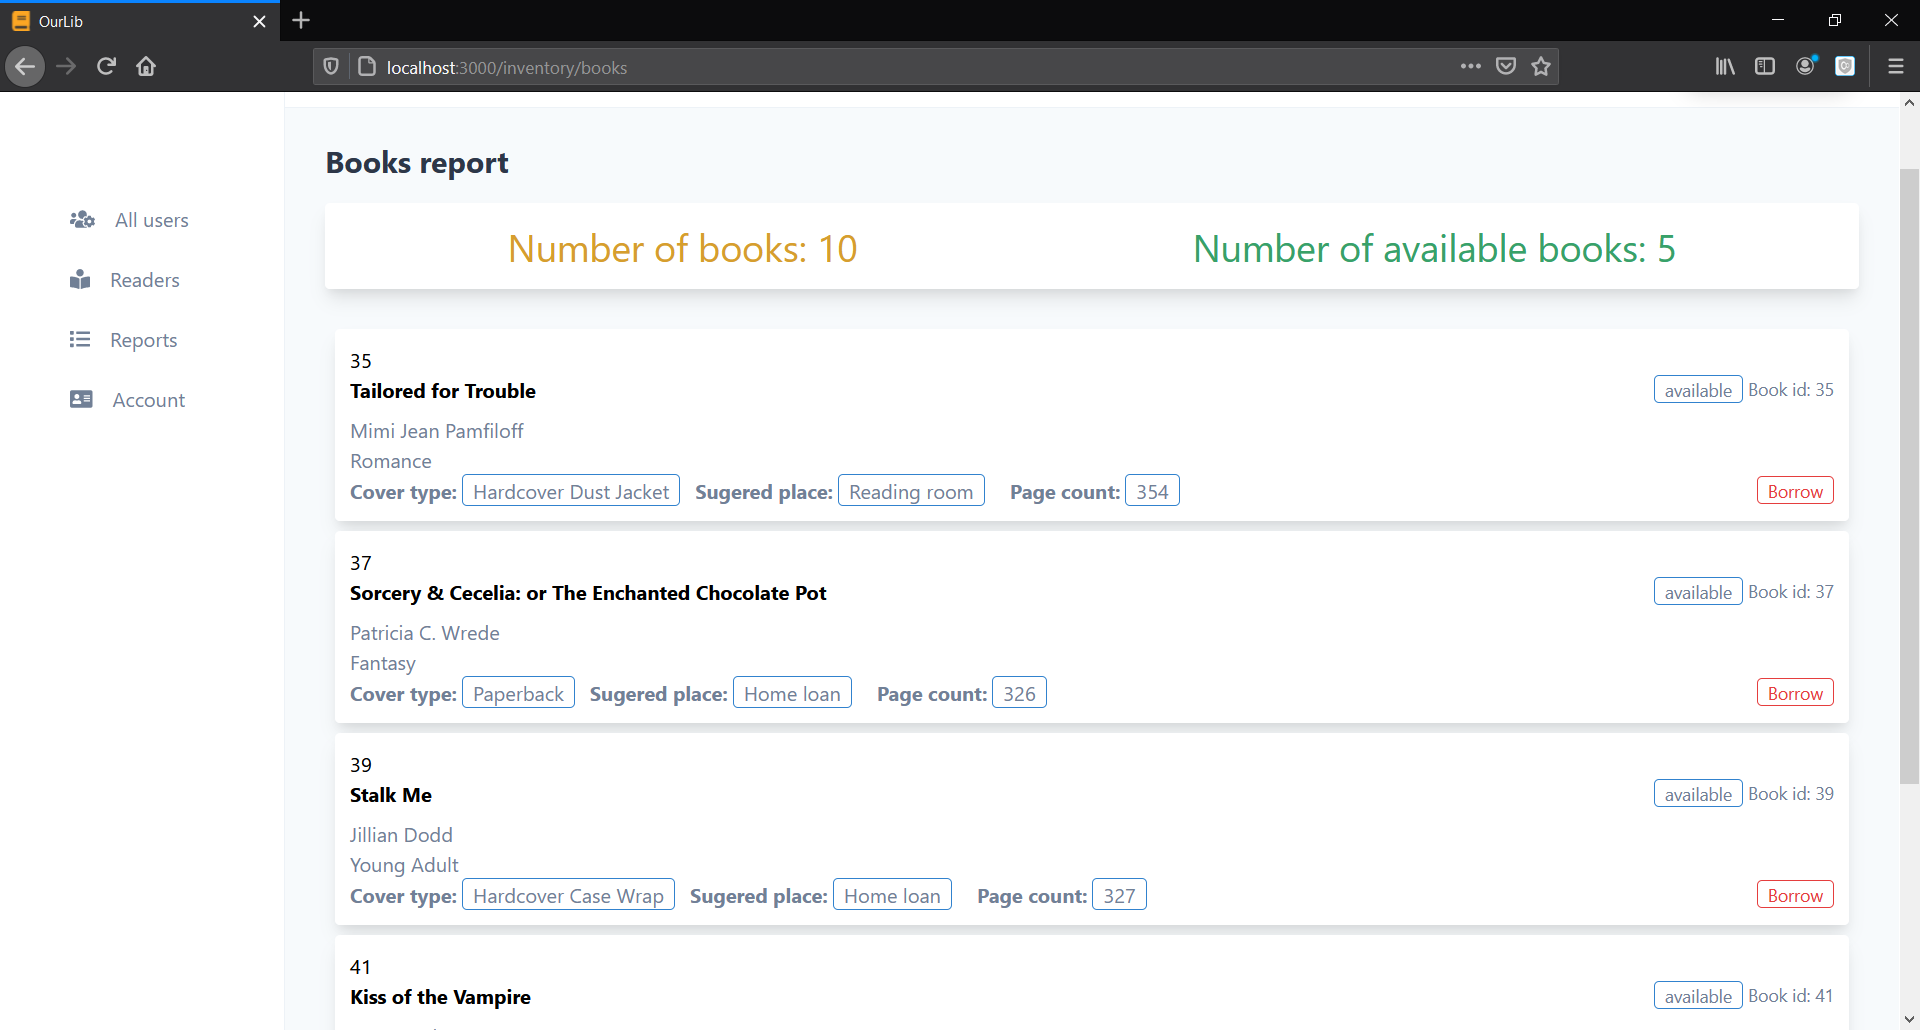
\includegraphics[width=\textwidth]{Include/Resources/FrontendScreens/React/adminBooksReports.png}
    \caption{Books in system report}
    \label{fig:ScreenshotGUIadminBooksReports}
\end{figure}




%%%%%%%%%%%%%%%%%%%%%%%%%%%%%%%%%%%%%%%%%
\begin{figure}[H]
    \centering
    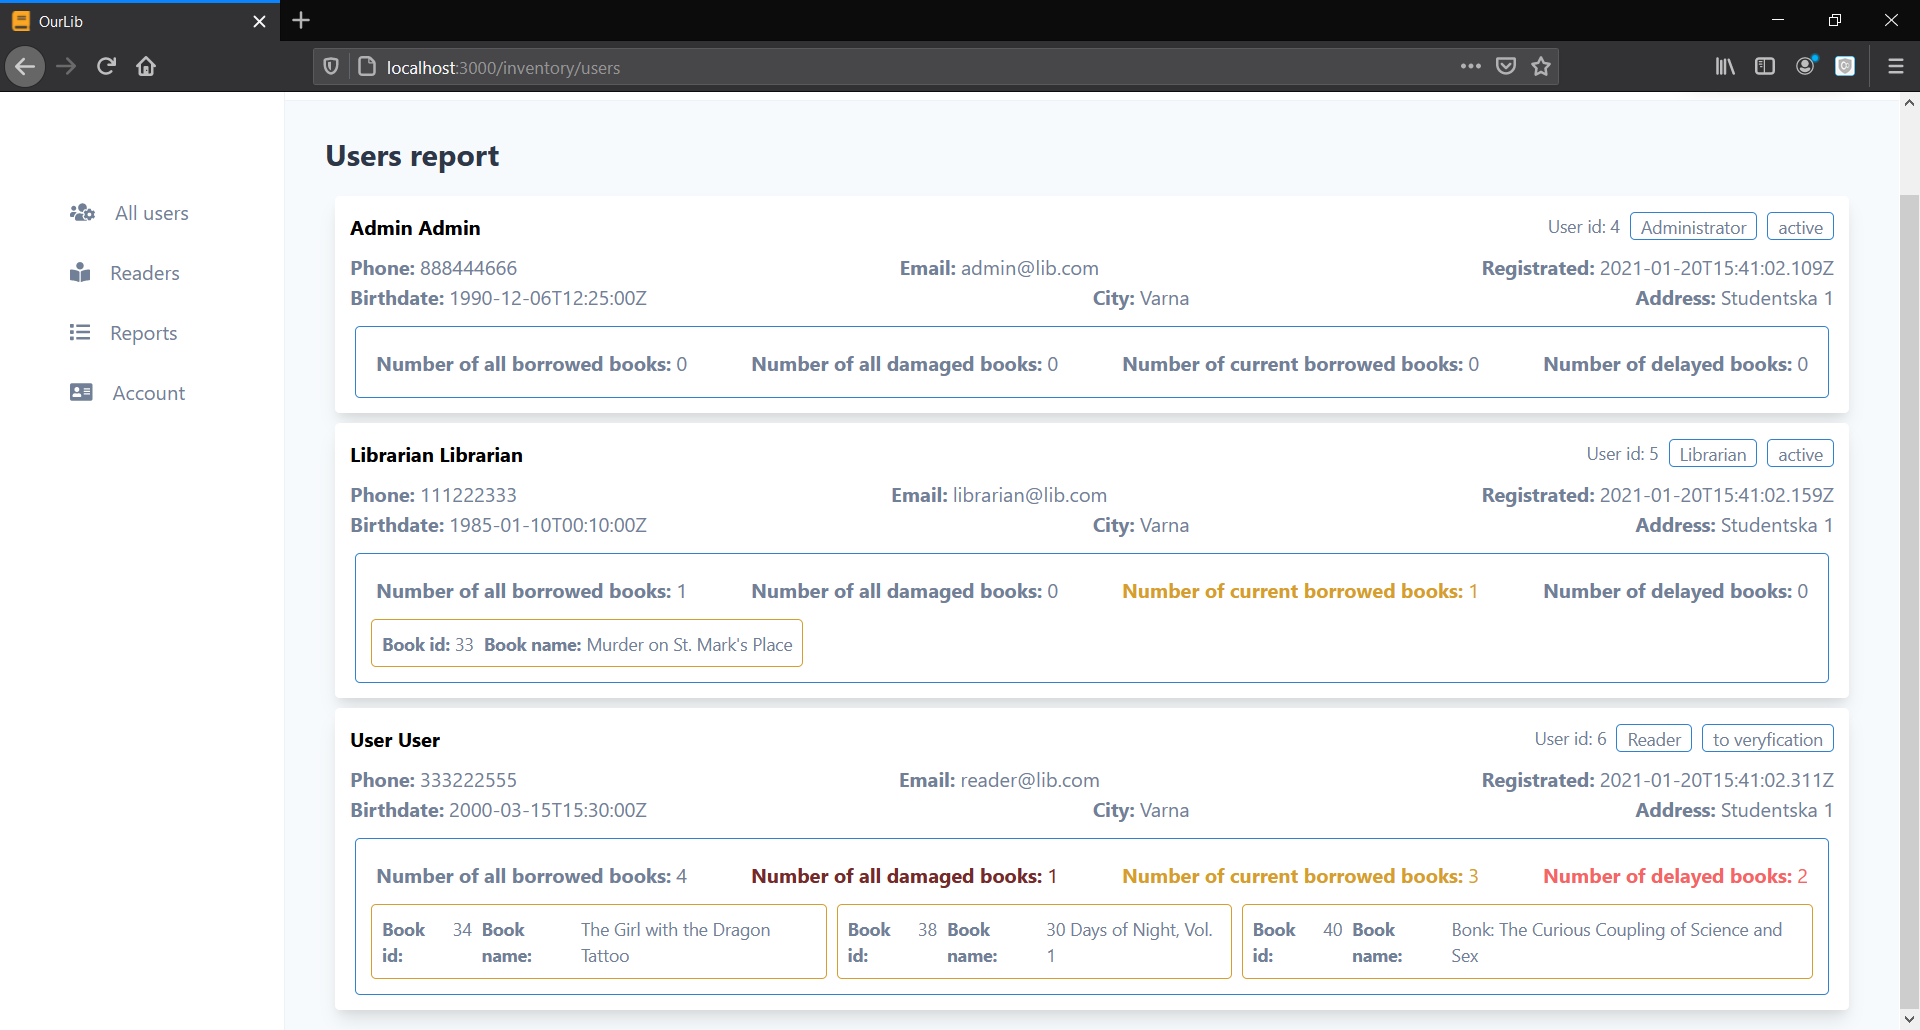
\includegraphics[width=\textwidth]{Include/Resources/FrontendScreens/React/adminUsersReport.png}
    \caption{Users in system report}
    \label{fig:ScreenshotGUIadminUsersReport}
\end{figure}



